% !TeX root = ../tfg.tex
% !TeX encoding = utf8

\chapter{Conceptos y estado del arte}

La \textbf{inteligencia artificial} (IA) se define en  \cite{russell2016artificial} como el campo de estudio de la informática que se centra en la creación de agentes inteligentes, es decir, sistemas que perciben su entorno y toman acciones que maximizan sus posibilidades de éxito en algún objetivo o tarea.

La inteligencia artificial abarca una amplia variedad de problemas y aplicaciones, entre los que destacan:

\begin{itemize}
	\item \textbf{Resolución de Problemas y Búsqueda}: La IA desarrolla algoritmos para encontrar soluciones óptimas o satisfactorias en espacios de búsqueda complejos. Esto incluye problemas clásicos como el ajedrez, el rompecabezas del cubo de Rubik o la planificación de rutas.
	
	\item \textbf{Representación del Conocimiento y Razonamiento}: Este área se centra en cómo representar información sobre el mundo de manera que un ordenador pueda utilizarla para resolver problemas complejos y tomar decisiones. Ejemplos incluyen sistemas expertos y razonamiento basado en casos.
	
	\item \textbf{Aprendizaje Automático}: Como veremos posteriormente, el aprendizaje automático se enfoca en el desarrollo de algoritmos que permitan a los ordenadores aprender a partir de los datos y mejorar con la experiencia.
	
	\item \textbf{Procesamiento del Lenguaje Natural (NLP)}: El NLP busca permitir que los ordenadores comprendan, interpreten y respondan al lenguaje humano de manera útil. Algunas aplicaciones de este campo incluyen la traducción automática, el análisis de sentimientos y la implementación de agentes conversacionales.
	
	\item \textbf{Visión Artificial}: Este campo se enfoca en que los ordenadores sean capaces de interpretar y comprender el contenido de imágenes y vídeos. Aplicaciones incluyen el reconocimiento facial, la conducción autónoma y la detección de objetos.
	
	\item \textbf{Robótica}: La IA aplicada a la robótica busca diseñar agentes que interactúen con el mundo físico. Esto incluye tareas como la navegación, la manipulación de objetos y la interacción humano-robot.
\end{itemize}

Es importante destacar que los problemas que aborda la inteligencia artificial pueden involucrar múltiples áreas. Por ejemplo, un sistema de conducción autónoma requiere la integración de visión artificial para interpretar el entorno, aprendizaje automático para mejorar su desempeño a partir de la experiencia y toma de decisiones, y algoritmos de planificación para determinar la mejor ruta a seguir. Esta interrelación de diferentes áreas y técnicas permite a los sistemas de IA abordar problemas complejos y dinámicos de manera más eficaz.

\section{Aprendizaje automático}

El \textbf{aprendizaje automático}  o \textbf{\textit{machine learning}} es la subdisciplina de la IA que se centra en el desarrollo de algoritmos y técnicas que permiten a los ordenadores aprender y hacer predicciones o tomar decisiones basadas en datos. Esta capacidad de aprendizaje se logra a través de la construcción de modelos que pueden mejorar su rendimiento en tareas específicas mediante la experiencia y los datos disponibles. Este enfoque supuso un cambio de paradigma respecto al diseño de algoritmos tradicional, donde su desempeño dependía explícitamente del conocimiento sobre el problema de los ingenieros que lo implementaban.

Existen varios paradigmas del aprendizaje automático en función del nivel de supervisión humana necesaria durante el proceso de aprendizaje. Los tres tipos principales son:

\begin{itemize}
	\item \textbf{Aprendizaje Supervisado}: En este tipo, el algoritmo aprende a partir de un conjunto de datos etiquetados. Cada ejemplo en el conjunto de datos incluye una entrada y una salida esperada. El objetivo es que el modelo aprenda a identificar las salidas correctas a partir de las entradas para poder hacer predicciones sobre datos nuevos. Aplicaciones comunes incluyen la clasificación y la regresión.
	
	\item \textbf{Aprendizaje No Supervisado}: A diferencia del aprendizaje supervisado, en el aprendizaje no supervisado los datos no están etiquetados. El objetivo es descubrir estructuras o patrones ocultos en los datos. Las técnicas de agrupamiento o \textit{clustering}, y la reducción de dimensionalidad son ejemplos comunes de aprendizaje no supervisado.
	
	\item \textbf{Aprendizaje por Refuerzo}: En este enfoque, un agente aprende a tomar decisiones mediante la interacción con un entorno dinámico. El agente recibe recompensas o penalizaciones en función de las acciones que realiza, y su objetivo es maximizar la recompensa acumulada a lo largo del tiempo. Este tipo de aprendizaje es especialmente útil en problemas de toma de decisiones secuenciales, como en juegos y robótica.
\end{itemize}

El aprendizaje automático se utiliza para abordar una amplia variedad de problemas en diferentes dominios. Algunos de los problemas más destacados incluyen:

\begin{itemize}
	\item \textbf{Clasificación}: El objetivo de la clasificación es asignar una etiqueta a una entrada entre un conjunto de etiquetas posibles. Ejemplos de problemas de clasificación incluyen el reconocimiento de imágenes, el filtrado de spam y el diagnóstico médico.
	
	\item \textbf{Regresión}: La regresión se centra en predecir un valor continuo a partir de una entrada. Un ejemplo clásico es la predicción de precios de viviendas basándose en características como el tamaño y la ubicación.
	
	\item \textbf{Agrupamiento (\textit{Clustering})}: Este problema implica agrupar un conjunto de datos en subconjuntos, o clusters, de tal manera que los datos en el mismo \textit{cluster} sean más similares entre sí que con los datos de otros \textit{clusters}. Aplicaciones incluyen segmentación de mercado y análisis de imágenes.
	
	\item \textbf{Reducción de Dimensionalidad}: La reducción de dimensionalidad se utiliza para simplificar modelos complejos reduciendo el número de variables en el análisis de datos. Técnicas como el Análisis de Componentes Principales (PCA) o \textit{Locally Linear Embedding} (LLE) son comunes en este campo.
	
	\item \textbf{Detección de Anomalías}: También conocido como detección de \textit{outliers}, este problema implica identificar datos que no se ajustan al comportamiento normal esperado. Es crucial en áreas como la detección de fraudes y el monitoreo de sistemas.
\end{itemize}

El avance en el aprendizaje automático ha llevado a desarrollos significativos en múltiples campos, transformando la manera en que se analizan los datos y se toman decisiones en el mundo real.

\section{Visión artificial}

Como hemos comentado anteriormente de manera breve, la \textbf{visión artificial} es la rama de la IA cuyo objetivo es comprender el mundo que percibimos a partir de una o más imágenes y reconstruir propiedades suyas como su forma, iluminación o distribución de colores. Su objetivo final es desarrollar sistemas que puedan interpretar y comprender el entorno visual de manera efectiva.

La \textbf{visión artificial} es un campo muy diverso que integra métodos de varias áreas del conocimiento para lograr su objetivo principal. Como resultado, abarca una amplia gama de aplicaciones y tareas. Algunas de las más destacadas incluyen:

\begin{itemize} 
	\item \textbf{Clasificación de objetos}: identificar y categorizar objetos en una imagen, lo que es fundamental en aplicaciones como la detección de objetos en imágenes de seguridad o la clasificación de productos en una tienda en línea. 
	\item \textbf{Generación de imágenes}: crear imágenes a partir de modelos o datos, lo que tiene aplicaciones en la creación de gráficos 3D, la síntesis de imágenes para la publicidad o la creación de contenido en redes sociales. 
	\item \textbf{Reconstrucción de entornos 3D}: reconstruir entornos tridimensionales a partir de imágenes 2D, lo que es fundamental en aplicaciones como la creación de modelos 3D de edificios o la planificación de rutas en un entorno desconocido. 
	\item \textbf{Detección de objetos}: detectar la presencia de objetos en una imagen, lo que es fundamental en aplicaciones como la seguridad en espacios públicos o la detección de anomalías en la producción industrial. 
	\item \textbf{Segmentación de imágenes}: dividir una imagen en regiones significativas, lo que es fundamental en aplicaciones como la medicina, la agricultura o la minería. 
\end{itemize}

La visión artificial es un campo en constante evolución que se ha desarrollado significativamente en las últimas décadas, al punto de haber superado a los seres humanos en ciertas aplicaciones específicas, como el reconocimiento de imágenes y la detección de objetos. Sin embargo, aún quedan numerosos desafíos por abordar, especialmente en contextos más complejos y variados, como la interpretación de escenas en tiempo real y la comprensión de imágenes en condiciones adversas.

\section{Redes neuronales artificiales}

Dentro de los distintos modelos de aprendizaje automático, nosotros trabajaremos con redes neuronales artificiales. Para entender mejor su funcionamiento, primero hablaremos de las neuronas biológicas y su inspiración en los modelos artificiales.

\subsection{Neuronas biológicas}

Las neuronas biológicas son células especializadas del sistema nervioso que desempeñan roles clave en la recepción, procesamiento y transmisión de señales. Estas células son fundamentales para la comunicación neuronal, permitiendo el flujo de información a través de complejas redes en el cerebro y otros componentes del sistema nervioso.

Las neuronas biológicas están compuestas por tres partes principales: el \textbf{soma}, que es el cuerpo celular conteniendo el núcleo y orgánulos celulares; las \textbf{dendritas}, extensiones que reciben señales de otras neuronas; y el \textbf{axón}, una prolongación especializada que conduce los potenciales de acción desde el soma hasta las terminaciones sinápticas. Estas terminaciones sinápticas se encuentran en las sinapsis, donde se produce la transmisión de señales a otras neuronas o tejidos.

\begin{figure}[H]
	\centering
	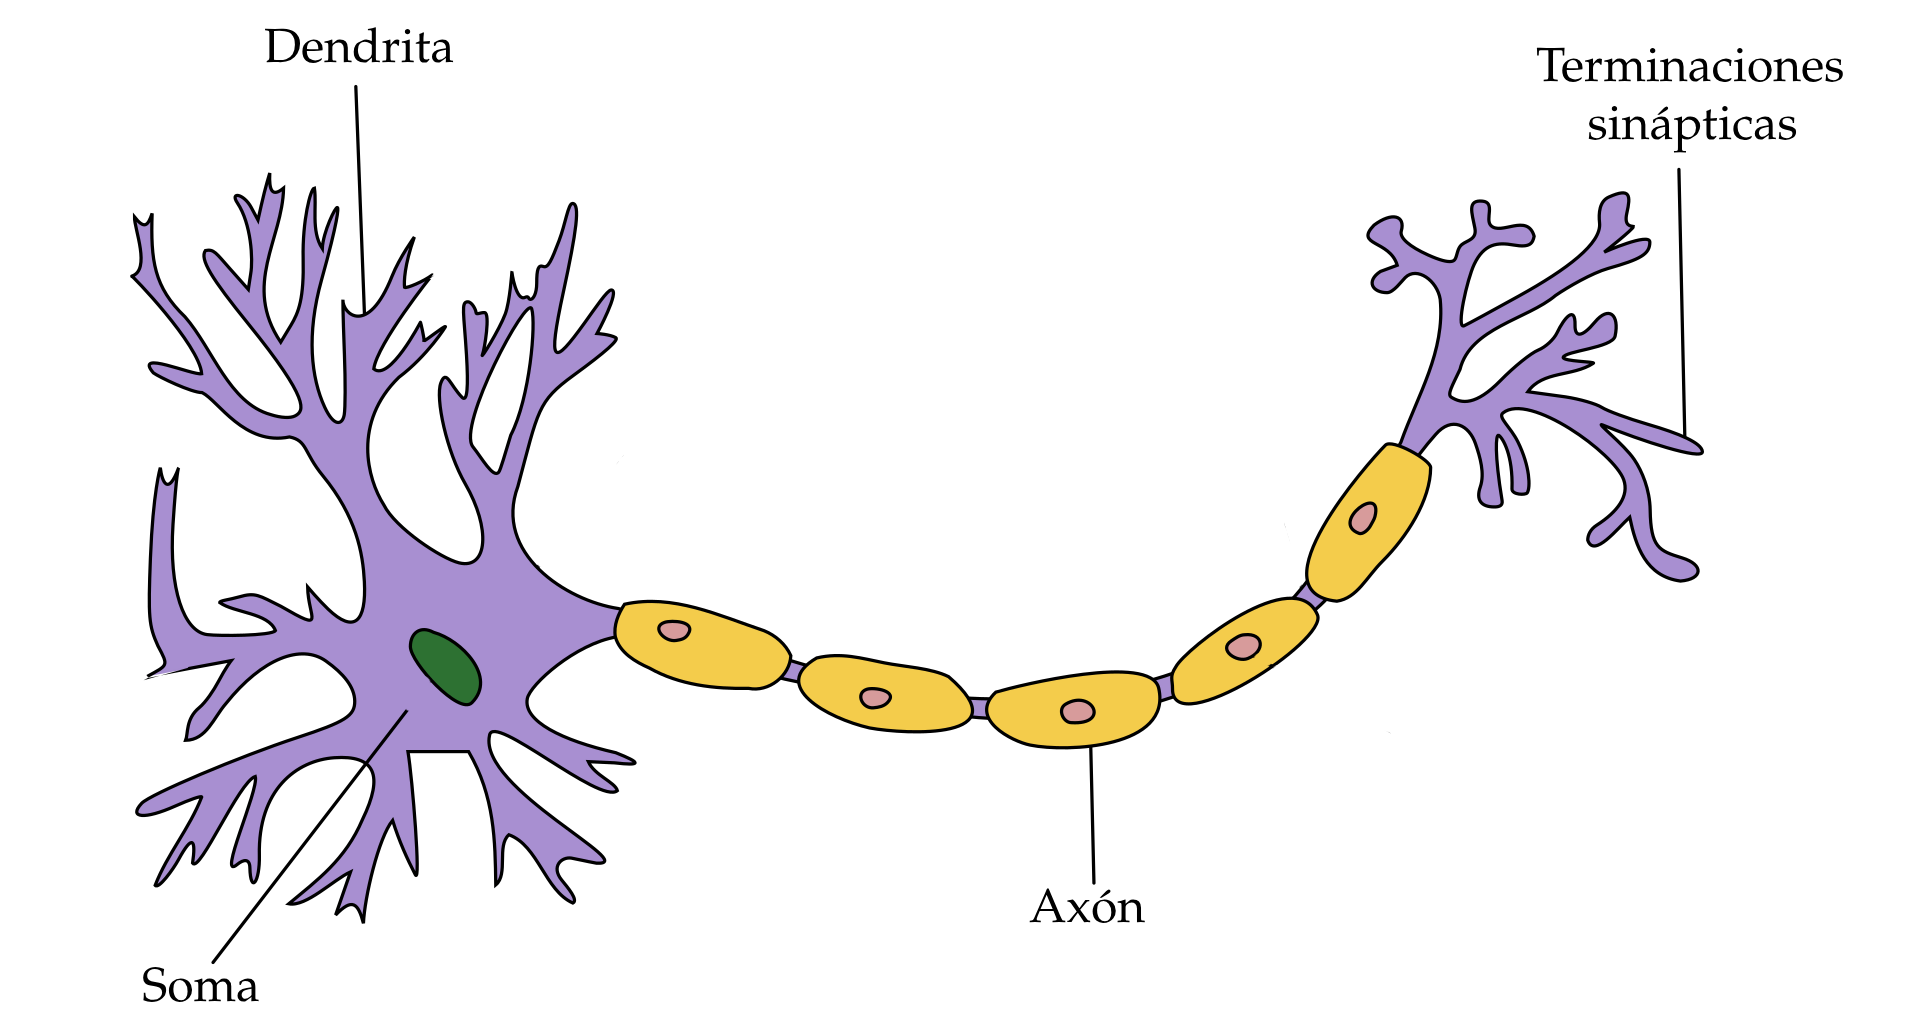
\includegraphics[width=100mm,scale=0.5]{img/neuron.png}
	\caption{Representación esquemática de una neurona biológica, mostrando el soma, las dendritas y el axón.}
\end{figure}

Esta compleja red de conexiones y la regulación electroquímica hacen que las neuronas biológicas sean fundamentales para coordinar y ejecutar numerosas funciones, desde simples reflejos hasta procesos cognitivos avanzados.

\subsection{Redes neuronales artificiales}

Las \textbf{neuronas artificiales} se inspiran en las neuronas biológicas en el sentido de que ambas tienen la capacidad de recibir, procesar y transmitir señales. En el caso de las neuronas artificiales, estas reciben señales de otras neuronas dentro de una red y las procesan mediante una combinación lineal de una matriz de \textbf{pesos} ajustables \(\mathbf{W}\) y un vector de \textbf{sesgo} o \textbf{\textit{bias}} \(\mathbf{b}\). Durante el entrenamiento de la red, estos parámetros se refinan para optimizar el rendimiento de la red en tareas específicas como clasificación o regresión. Cada neurona artificial aplica una función escalar denominada \textbf{función de activación} \(\theta: \mathbb{R}^m \to \mathbb{R}\), que transforma la combinación lineal de sus entradas:

\[
f(\mathbf{x}, \mathbf{W}, \mathbf{b}) = \theta(\mathbf{W}\mathbf{x} + \mathbf{b}), \quad \forall \mathbf{x} \in \mathbb{R}^d, \mathbf{W} \in \mathbb{R}^{m \times d}, \mathbf{b} \in \mathbb{R}^m.
\]

Donde \(d\) es la dimensión de entrada y \(m\) es el número de neuronas en la capa.

Estas neuronas se agrupan en \textbf{capas} dentro de una \textbf{red neuronal artificial} (ANN). La estructura de la red se define por su \textbf{profundidad}, que corresponde al número de capas ocultas, y su \textbf{anchura}, que se refiere al número de neuronas en cada capa.

\begin{figure}
	\centering
	\def\layersep{2.5cm}
	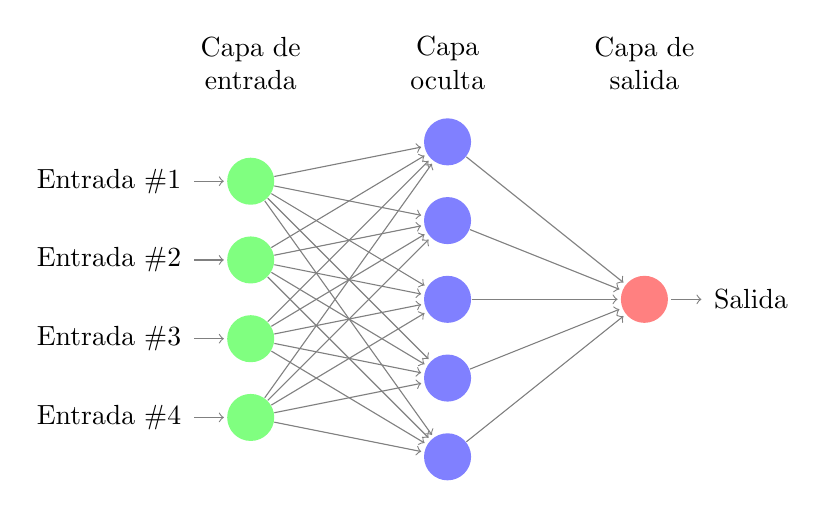
\begin{tikzpicture}[shorten >=1pt,->,draw=black!50, node distance=\layersep]
		\tikzstyle{every pin edge}=[<-,shorten <=1pt]
		\tikzstyle{neuron}=[circle,fill=black!25,minimum size=17pt,inner sep=0pt]
		\tikzstyle{input neuron}=[neuron, fill=green!50];
		\tikzstyle{output neuron}=[neuron, fill=red!50];
		\tikzstyle{hidden neuron}=[neuron, fill=blue!50];
		\tikzstyle{annot} = [text width=4em, text centered]
		
		% Draw the input layer nodes
		\foreach \name / \y in {1,...,4}
		% This is the same as writing \foreach \name / \y in {1/1,2/2,3/3,4/4}
		\node[input neuron, pin=left:Entrada \#\y] (I-\name) at (0,-\y) {};
		
		% Draw the hidden layer nodes
		\foreach \name / \y in {1,...,5}
		\path[yshift=0.5cm]
		node[hidden neuron] (H-\name) at (\layersep,-\y cm) {};
		
		% Draw the output layer node
		\node[output neuron,pin={[pin edge={->}]right:Salida}, right of=H-3] (O) {};
		
		% Connect every node in the input layer with every node in the
		% hidden layer.
		\foreach \source in {1,...,4}
		\foreach \dest in {1,...,5}
		\path (I-\source) edge (H-\dest);
		
		% Connect every node in the hidden layer with the output layer
		\foreach \source in {1,...,5}
		\path (H-\source) edge (O);
		
		% Annotate the layers
		\node[annot,above of=H-1, node distance=1cm] (hl) {Capa oculta};
		\node[annot,left of=hl] {Capa de entrada};
		\node[annot,right of=hl] {Capa de salida};
	\end{tikzpicture}
	\caption{Estructura de una FNN. Muestra una red neuronal hacia adelante con tres tipos de capas: entrada (verde), oculta (azul), y salida (rojo). Cada neurona de la capa de entrada está conectada a todas las neuronas en la capa oculta, demostrando un ejemplo de capas totalmente conectadas.}
\end{figure}

En el caso de las \textbf{redes neuronales hacia adelante} o \textbf{\textit{feedforward networks}} (FNNs), la red está compuesta por varias capas cuyas neuronas solamente están conectadas a neuronas en capas posteriores. En el caso donde todas las salidas de una capa están conectadas a todas las neuronas de la siguiente capa se les conoce como \textbf{capas totalmente conectadas} o \textbf{\textit{fully connected layers}} (FC). Las funciones de cada capa en una FNN pueden describirse como:

\[
f_j(\mathbf{x}) = \theta \left( \mathbf{W}_j \mathbf{x} + \mathbf{b}_j \right),
\]

donde \( \mathbf{W}_j \) es la matriz de pesos y \( \mathbf{b}_j \) es el vector de sesgo para la capa \( j \). Estos elementos son fundamentales para determinar cómo se transforman las entradas en salidas que serán utilizadas por la siguiente capa. La estructura funcional de las FNNs se describe entonces mediante la composición de estas funciones organizadas en capas:

\[
\nu = s \circ f_l \circ f_{l-1} \circ \ldots \circ f_2 \circ f_1(\mathbf{x}),
\]

donde \( l \) denota el número total de capas. La última capa de la red utiliza una función de activación \( s \), que convierte la salida de la capa final en uno o varios valores en función de la tarea designada a la red. Esta función de salida es crítica para aplicaciones como clasificación, donde el resultado necesita expresarse como una probabilidad, o para regresión, donde se ajusta a un rango específico.

\subsection{Funciones de activación}

Las funciones de activación son de gran importancia en la arquitectura de las ANNs, ya que introducen no linealidades en el modelo, permitiendo a la red aprender y modelar relaciones complejas en los datos. Sin estas funciones, la red no podría resolver tareas más complejas que una simple regresión lineal.

Anteriormente, hemos definido las funciones de activación en un contexto vectorial, aplicando una única transformación a todas las entradas procedentes de la capa anterior. Sin embargo, en la práctica es habitual emplear una función de activación escalar \(\theta : \mathbb{R} \rightarrow I\), donde \(I\) es un intervalo específico, de forma que se aplica componente a componente a cada combinación lineal de entrada.

Una de las funciones de activación más antiguas es la \textbf{sigmoide}, que se define como:
\begin{equation}
	\theta(z) = \frac{1}{1 + e^{-z}},
\end{equation}
donde \( \theta : \mathbb{R} \to [0,1] \) y \( z \) es la combinación lineal de entradas, pesos y sesgo de la neurona. La función sigmoide transforma los valores de entrada a un rango entre \(0\) y \(1\), modelando de esta forma probabilidades. Aunque su uso ha disminuido en redes profundas debido al problema del \textbf{desvanecimiento del gradiente}, problema que consiste en que los gradientes van disminuyendo progresivamente conforme profundizan en las capas de la red, impidiendo así su actualización. A pesar de ello, sigue siendo relevante en la capa de salida de ANNs para clasificación binaria.

La función \textbf{Softmax} es una generalización de la sigmoide para múltiples clases y se define para un vector \( z \in \mathbb{R}^K \) como:
\begin{equation}
	\theta(z)_i = \frac{e^{z_i}}{\sum_{k=1}^K e^{z_k}} \quad \text{para } i = 1, \ldots, K,
\end{equation}
donde \( \theta : \mathbb{R}^K \to [0,1]^K \). Cada componente de la salida, \(\theta(z)_i\), representa la probabilidad de que la entrada pertenezca a la clase \(i\), y se utiliza principalmente en la capa de salida de las redes neuronales para tareas de clasificación multiclase.

La \textbf{tangente hiperbólica} (\(\tanh\)), que se define como:
\begin{equation}
	\theta(z) = \tanh(z) = \frac{2}{1 + e^{-2z}} - 1,
\end{equation}
donde \( \theta : \mathbb{R} \to [-1,1] \), es preferida sobre la sigmoide en algunos escenarios por su salida centrada en cero, que facilita la optimización durante el entrenamiento. Aunque también sufre del problema de desvanecimiento de gradiente, su uso en capas ocultas es bastante frecuente.

La \textbf{\textit{Rectified Linear Unit}} (ReLU), definida como:
\begin{equation}
	\theta(z) = \max(0, z),
\end{equation}
donde \( \theta : \mathbb{R} \to [0, \infty) \), es la más utilizada en aprendizaje profundo por su simplicidad y eficiencia computacional. ReLU se utiliza generalmente en capas ocultas, pero no es adecuada para la capa de salida en tareas de clasificación debido a su rango no acotado. Además, ReLU sufre de un problema de "\textbf{muerte de neuronas}" o "\textbf{\textit{dying ReLU}}", que sucede cuando los valores de entrada son menores o iguales a cero. Debido a que la salida de ReLU es cero para estos valores, los gradientes también son cero durante la retropropagación. Como resultado, estas neuronas dejan de aprender y contribuyen poco o nada al modelo, afectando negativamente el rendimiento de la red.

La \textbf{\textit{Leaky ReLU}} es una variante de la ReLU definida como:
\begin{equation}
	\theta(z) = \max(\alpha z, z),
\end{equation}
donde \( \alpha \) es un coeficiente real positivo y \( \theta : \mathbb{R} \to \mathbb{R} \). Esta función se utiliza también en capas ocultas para evitar la muerte de neuronas que puede ocurrir con ReLU.

%
%La \textbf{Gaussian Error Linear Unit} (GELU) es una función de activación que se inspira en probabilidades y es utilizada principalmente en modelos de procesamiento de lenguaje natural, aunque su aplicación se ha extendido a otras áreas de aprendizaje profundo. La GELU se define como:
%\begin{equation}
%	\theta(z) = z \cdot \Phi(z),
%\end{equation}
%donde \(\Phi(z)\) es la función de distribución acumulativa de una distribución normal estándar y \(\theta : \mathbb{R} \to \mathbb{R}\). Esta función de activación modula la salida de la neurona de una manera no lineal y adaptativa, permitiendo que la activación sea ponderada por la probabilidad de que z sea positivo en una distribución gaussiana. Este enfoque ofrece un compromiso entre linealidad y no linealidad, permitiendo que la red adapte mejor sus activaciones a la distribución de los datos, lo cual ha demostrado ser efectivo en mejorar la capacidad de generalización del modelo.
%
Finalmente tenemos la \textbf{\textit{Sigmoid Linear Unit}} (SiLU), también conocida como \textbf{Swish}, es una de las funciones de activación más recientes que combina elementos de la función sigmoide y linealidad. Se define como:
\begin{equation}
	\theta(z) = \frac{z}{1 + e^{-z}},
\end{equation}
donde \(\theta : \mathbb{R} \to \mathbb{R}\). A diferencia de la ReLU y sus variantes, la SiLU permite que valores negativos tengan una contribución, aunque moderada, a la activación, lo que resulta en una capacidad mejorada para ajustar gradientes durante el entrenamiento. Esta característica hace que la SiLU sea particularmente útil en capas profundas de redes neuronales. Esta función ha mostrado ventajas en términos de rendimiento de convergencia y eficacia en comparación con funciones más tradicionales \cite{ramachandran2017searching}.

Cada una de estas funciones de activación juega un papel crucial en la arquitectura de una red neuronal, y la elección de una sobre otra puede depender del problema específico que se esté abordando, del comportamiento de la red durante el entrenamiento y de la naturaleza de los datos.

\begin{figure}
	\centering
	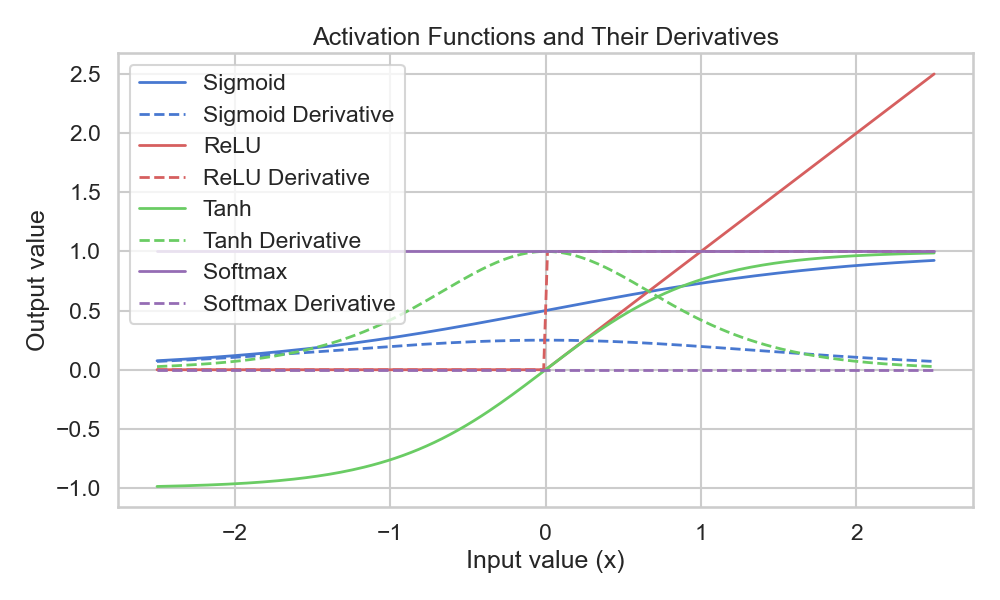
\includegraphics[width=12cm]{img/activation_functions_figure.png}
	\caption{Figura}
\end{figure}

\subsection{Optimización en redes neuronales}

El entrenamiento de estas redes se realiza mediante el uso de métodos de optimización que ajustan iterativamente los parámetros de la red para minimizar una función denominada \textbf{función de pérdida} o \textbf{coste}, denotada por \(\mathcal{L}\). Esta función evalúa la diferencia entre las salidas predichas por la red \(\mathbf{\hat{y}}\) y los valores reales o esperados \(\mathbf{y}\).

Una elección típica de función de pérdida en tareas de clasificación multiclase es la \textbf{entropía cruzada} o \textbf{\textit{cross entropy}}, que se utiliza en combinación con la función de activación \textbf{Softmax}. Softmax se aplica en la última capa de la red para convertir las salidas lineales en un vector de probabilidades que suman uno, siendo cada componente $i$ la evaluación de Softmax en la respectiva clase. De esta forma,

\[
\mathbf{\hat{y}} = \text{Softmax}(\mathbf{z}) = \left(\frac{e^{z_1}}{\sum_{j=1}^{N} e^{z_j}}, \frac{e^{z_2}}{\sum_{j=1}^{N} e^{z_j}}, \ldots, \frac{e^{z_N}}{\sum_{j=1}^{N} e^{z_j}}\right),
\]

donde \(\mathbf{z}\) representa las salidas de la última capa de la red antes de la aplicación de Softmax. Con el vector de probabilidades establecido por Softmax, la entropía cruzada se calcula entonces como:

\[
\mathcal{L}(\mathbf{y}, \mathbf{\hat{y}}) = -\sum_{i=1}^{N} y_i \log(\hat{y}_i),.
\]

Aquí, \(\mathbf{y} = (y_1, y_2, \ldots, y_N)\) es el vector de etiquetas reales en formato \textit{one-hot}, donde \(y_i = 1\) si la clase \(i\) es la correcta y \(y_i = 0\) en caso contrario. Cada elemento \(\hat{y}_i\) en \(\mathbf{\hat{y}}\) indica la probabilidad predicha de que la entrada pertenezca a la clase \(i\), y la suma de todas las probabilidades es igual a uno. La función de entropía cruzada mide entonces la diferencia entre las distribuciones de las etiquetas reales y las probabilidades predichas, y su minimización lleva al modelo a mejorar la precisión de sus predicciones.

En el ámbito del aprendizaje profundo también es común notar la función de pérdida como \(\mathcal{L}(\mathcal{W};\mathbf{x}, \mathbf{y})\), siendo \(\mathcal{W}\) el conujnto de pesos de la red y \(\mathbf{x}\) el vector de entrada, de forma que \(\mathcal{L}(\mathcal{W};\mathbf{x}, \mathbf{y}) = \mathcal{L}(\nu(\mathbf{x}), \mathbf{y})\).

El principal método de entrenamiento de redes neuronales consta de dos pasos: el \textbf{paso hacia adelante} o \textbf{\textit{forward pass}}, que calcula la salida de la red a partir de la entrada; y la \textbf{propagación hacia atrás}, también conocida como \textbf{retropropagación} o \textbf{\textit{backpropagation}}. Este algoritmo es un método para calcular el gradiente de la función de pérdida con respecto a cada parámetro de la red aplicando la regla de la cadena. Este proceso se inicia en la capa de salida y se propaga hacia atrás a través de la red, de la siguiente manera:

\[
\frac{\partial \mathcal{L}}{\partial w_{ij}^{(l)}} = \frac{\partial \mathcal{L}}{\partial x_i^{(l+1)}} \cdot \frac{\partial x_i^{(l+1)}}{\partial z_i^{(l+1)}} \cdot \frac{\partial z_i^{(l+1)}}{\partial w_{ij}^{(l)}},
\]

donde \( \mathcal{L} \) es la función de pérdida, \( w_{ij}^{(l)} \) son los pesos de la capa \( l \), \( x_i^{(l+1)} \) es la salida de la neurona \( i \) en la capa \( l+1 \), y \( z_i^{(l+1)} \) es la entrada en forma de combinación lineal a la neurona \( i \) en la capa \( l+1 \), que se calcula como \( z_i^{(l+1)} = \sum_j w_{ij}^{(l)} x_j^{(l)} + b_i^{(l)} \). La derivada \(\frac{\partial x_i^{(l+1)}}{\partial z_i^{(l+1)}}\) es la derivada de la función de activación \(\theta\) aplicada a \( z_i^{(l+1)} \).

Como los métodos de optimización que emplearemos están basados en el cálculo del gradiente, restringiremos la optimización a los vectores de pesos \(\mathbf{w}\) en las distintas capas. En consecuencia, definiremos la función a optimizar como \textbf{función objetivo} \(J\) tal que \(J(\mathcal{W}) = \mathcal{L}(\mathcal{W};\mathbf{x}, \mathbf{y})\). Sin embargo, por comodidad abusaremos de la notación y escribiremos el gradiente de \(J\) respecto al vector \(\mathbf{w}\), \(\nabla_{\mathbf{w}} J(\mathcal{W})\), simplemente por \(\nabla J(\mathbf{w})\).

La optimización efectiva de estos pesos es crucial para el rendimiento de la red, y se lleva a cabo a través de varias iteraciones de entrenamiento, ajustando progresivamente los parámetros para reducir el error y mejorar la precisión de la clasificación o la predicción de la red.

\subsubsection{Descenso del gradiente}

El algoritmo de \textbf{descenso del gradiente} \cite{cauchy1847methode} es el enfoque más básico de optimización, donde los pesos se actualizan en la dirección opuesta al gradiente de la función objetivo:
\begin{equation}
	\mathbf{w}_{\text{nuevo}} = \mathbf{w}_{\text{viejo}} - \alpha \nabla J (\mathbf{w}_{\text{viejo}}),
\end{equation}
donde \(\alpha\) representa la \textbf{tasa de aprendizaje} y \(\nabla J (\mathbf{w}_{\text{viejo}})\) es el gradiente de la función de pérdida con respecto a los pesos anteriores. El descenso del gradiente puede implementarse de varias maneras dependiendo de cómo se seleccionan y utilizan los datos para calcular el gradiente de la función de pérdida. Una forma es el \textbf{descenso del gradiente estocástico} (SGD), que actualiza el conjunto de pesos después de cada ejemplo de entrenamiento, siendo muy utilizado en grandes conjuntos de datos. Otra variante es el \textbf{descenso del gradiente por lotes}, que calcula el gradiente utilizando todo el conjunto de datos antes de realizar una actualización, asegurando una actualización consistente de los pesos. Finalmente, el \textbf{descenso del gradiente por mini-lotes} divide el conjunto de datos en pequeños lotes y realiza actualizaciones de los pesos después de procesar cada mini-lote, combinando aspectos de las dos técnicas anteriores.

\subsubsection{Momentum}

Una técnica que mejora la eficacia del descenso del gradiente es el \textbf{\textit{momentum}} \cite{rumelhart1986learning}, que ayuda a acelerar el algoritmo en la dirección correcta mientras suaviza las actualizaciones de pesos. En lugar de actualizar los pesos basándose únicamente en el gradiente actual, el \textit{momentum} también considera los gradientes anteriores para obtener una dirección más estable y consistente. Esto se logra mediante la introducción de una variable \(\mathbf{v}_t\), conocida como el \textbf{término de \textit{momentum}}, que acumula los gradientes pasados con un \textbf{factor de descuento} \(\gamma\), normalmente fijado entre 0.9 y 0.99. La fórmula de actualización con \textit{momentum} es entonces:
\begin{equation}
	\mathbf{v}_{t} = \gamma \mathbf{v}_{t-1} + \alpha \nabla J(\mathbf{w}_{\text{viejo}}),
\end{equation}
\begin{equation}
	\mathbf{w}_{\text{nuevo}} = \mathbf{w}_{\text{viejo}} - \mathbf{v}_{t},
\end{equation}
donde \(\alpha\) es la tasa de aprendizaje. Este enfoque no solo acelera la convergencia, sino que también puede ayudar a evitar los mínimos locales subóptimos, haciendo que el algoritmo sea más eficaz y robusto en práctica.


\subsubsection{Adagrad}

\textbf{\textit{Adaptative Gradient Algorithm}} (Adagrad) \cite{duchi2011adaptive} es un algoritmo de optimización que adapta individualmente la tasa de aprendizaje de cada parámetro basándose en la magnitud acumulada de sus gradientes. La actualización de los pesos \(\mathbf{w}\) se realiza mediante la siguiente fórmula:
\[
\mathbf{w}_{\text{nuevo}} = \mathbf{w}_{\text{viejo}} - \frac{\alpha}{\sqrt{\mathbf{G}^{(t)} + \epsilon}} \odot \nabla J(\mathbf{w}_{\text{viejo}}),
\]
donde \( \mathbf{G}^{(t)} \) es una matriz diagonal en la que cada elemento \( G_{ii}^{(t)} \) representa la suma acumulada de los cuadrados de las derivadas parciales de los gradientes con respecto a cada componente \( w_i \) de \(\mathbf{w}\) hasta el instante de tiempo \(t\). El \textbf{producto de Hadamard} \(\odot : \mathbb{R}^N \times \mathbb{R}^N \to \mathbb{R}^N\) se define como el producto escalar componente a componente. El término \( \epsilon \) es un pequeño valor constante añadido a cada elemento de \( \mathbf{G}^{(t)} \) para garantizar estabilidad numérica y evitar la división por cero. Cada elemento \( G_{ii}^{(t)} \) de la matriz se actualiza como sigue:
\[
G_{ii}^{(\text{nuevo})} = G_{ii}^{(\text{viejo})} + \left(\frac{\partial J}{\partial w_i} (\mathbf{w}_{\text{viejo}})\right)^2,
\]
permitiendo que las tasas de aprendizaje sean más bajas para parámetros con gradientes altos y mayores para aquellos con gradientes menores, lo cual facilita una convergencia más rápida y estable del algoritmo.

\subsubsection{RMSProp}

\textbf{\textit{Root Mean Square Propagation}} (RMSProp) \cite{hinton2012lecture} modifica Adagrad para mejorar su rendimiento manteniendo un promedio móvil del cuadrado de los gradientes. Esto ajusta la tasa de aprendizaje de manera más adecuada para problemas a largo plazo:
\begin{equation}
	\mathbf{v}_{t} = \beta \mathbf{v}_{t-1} + (1 - \beta) (\nabla J(\mathbf{w}_{\text{viejo}}))^2,
\end{equation}
\begin{equation}
	\mathbf{w}_{\text{nuevo}} = \mathbf{w}_{\text{viejo}} - \frac{\alpha}{\sqrt{\mathbf{v}_{t} + \epsilon}} \odot \nabla J(\mathbf{w}_{\text{viejo}}),
\end{equation}
donde \(\mathbf{v}_{t}\) es la media móvil del cuadrado de los gradientes y \(\beta\) es un factor de descuento que determina la ponderación de dicha media.

\subsubsection{Adam}

\textbf{\textit{Adaptive Moment Estimation}} (Adam) \cite{kingma2014adam} combina las ideas detrás de momentum y RMSprop. Mantiene estimaciones de los primeros y segundos momentos de los gradientes para ajustar la tasa de aprendizaje de cada parámetro de manera individual:
\begin{equation}
	\mathbf{m}_{t} = \beta_1 \mathbf{m}_{t-1} + (1 - \beta_1)\nabla J(\mathbf{w}_{\text{viejo}}),
\end{equation}
\begin{equation}
	\mathbf{v}_{t} = \beta_2 \mathbf{v}_{t-1} + (1 - \beta_2)(\nabla J(\mathbf{w}_{\text{viejo}}))^2,
\end{equation}
\begin{equation}
	\hat{\mathbf{m}}_{t} = \frac{\mathbf{m}_{t}}{1 - \beta_1^t},
\end{equation}
\begin{equation}
	\hat{\mathbf{v}}_{t} = \frac{\mathbf{v}_{t}}{1 - \beta_2^t},
\end{equation}
\begin{equation}
	\mathbf{w}_{\text{nuevo}} = \mathbf{w}_{\text{viejo}} - \frac{\alpha}{\sqrt{\hat{\mathbf{v}}_{t} + \epsilon}} \odot \hat{\mathbf{m}}_{t},
\end{equation}
donde \(\mathbf{m}_{t}\) y \(\mathbf{v}_{t}\) son estimaciones del primer y segundo momento respectivamente, \(\hat{\mathbf{m}}_{t}\) y \(\hat{\mathbf{v}}_{t}\) son sus correcciones sesgadas, y \(\beta_1\), \(\beta_2\) son tasas de decaimiento exponencial para los momentos estimados.

La selección del algoritmo de optimización es una decisión clave que puede variar dependiendo de la naturaleza del problema y el tipo de red neuronal que se está entrenando. SGD y Adam son especialmente populares debido a su robustez y buen desempeño en una amplia variedad de problemas. Sin embargo, la eficiencia de estos algoritmos no solo se debe a su diseño, sino también a la selección adecuada de hiperparámetros, como la tasa de aprendizaje y los coeficientes de momentum. Una tasa de aprendizaje mal configurada puede llevar al algoritmo a converger demasiado lentamente o a no converger en absoluto \cite{bottou2018optimization}. Por lo tanto, el ajuste fino de estos hiperparámetros, que a menudo requiere experimentación y experiencia, es importante para maximizar el rendimiento del modelo.

\subsection{Regularización de redes neuronales}

Un problema muy conocido en el ámbito del aprendizaje profundo es el \textbf{sobreajuste} u \textbf{\textit{overfitting}}, el cual ocurre cuando una red neuronal aprende patrones específicos del conjunto de entrenamiento en lugar de las verdaderas relaciones subyacentes entre los datos. Este fenómeno resulta en un rendimiento deficiente cuando la red se expone a datos nuevos y no vistos durante el entrenamiento. Para combatir el sobreajuste y mejorar la capacidad de generalización de las redes neuronales, se utilizan técnicas de \textbf{regularización}.

\subsubsection{Regularización $L1$ y $L2$}

Entre las técnicas más populares de regularización se encuentran la \textbf{regularización $\mathbf{L1}$ y $\mathbf{L2}$}, también conocidas como \textbf{\textit{Lasso}} y \textbf{\textit{Ridge}} respectivamente. Estas técnicas modifican la función objetivo añadiendo términos que penalizan los pesos grandes de la red.

La regularización $L1$, o \textit{Lasso}, añade a la función objetivo original $J(\mathbf{w})$ un término proporcional a la suma de los valores absolutos de los pesos:
\[
J_{L1}(\mathbf{w}) = J(\mathbf{w}) + \lambda \sum_{i} |w_i|,
\]
donde $\lambda$ es el parámetro de regularización. Este método es particularmente útil para generar modelos más interpretables al promover la \textbf{dispersión} o \textit{sparsity} de los pesos, lo que resulta en que algunos de ellos sean exactamente cero, reduciendo así la complejidad del modelo.

Por otro lado, la regularización $L2$, o \textit{Ridge}, añade un término proporcional a la suma de los cuadrados de los pesos:
\[
J_{L2}(\mathbf{w}) = J(\mathbf{w}) + \lambda \sum_{i} w_i^2.
\]
A diferencia de la regularización $L1$, la regularización $L2$ penaliza más agresivamente los valores grandes de los pesos, favoreciendo soluciones con pesos más uniformemente distribuidos y pequeños. Esto contribuye a una mejor generalización del modelo al desincentivar los pesos grandes, lo que lleva a soluciones más homogéneas y en consecuencia, a modelos que pueden generalizar mejor ante nuevos datos.

\subsubsection{Dropout}

\textbf{\textit{Dropout}} es otra técnica ampliamente utilizada que implica desactivar aleatoriamente una proporción de neuronas durante cada iteración del entrenamiento:
\begin{equation}
	x' = x \odot \mathcal{B}(p),
\end{equation}
donde $x$ es la salida de la función de activación de una capa y $\mathcal{B}(p)$ es un vector binario aleatorio donde cada elemento tiene una probabilidad $p \in [0,1]$ de ser cero. Esta técnica reduce el sobreajuste al forzar a la red a aprender representaciones redundantes.

\subsubsection{Early stopping}

El \textbf{\textit{early stopping}} es una técnica de regularización diseñada para prevenir el sobreajuste al detener el entrenamiento de un modelo de aprendizaje automático antes de que se manifieste el sobreajuste. Este método consiste en monitorear el rendimiento del modelo en un conjunto de validación separado durante el entrenamiento. Si el error de validación no solo comienza a incrementar, sino que lo hace por un margen mayor a un \textbf{umbral} definido \(\delta\), entonces indica que el modelo está empezando a aprender el ruido y las particularidades del conjunto de entrenamiento en lugar de las relaciones generales, por lo que el entrenamiento se detiene. La implementación de \textit{early stopping} requiere definir otro hiperparámetro comunmente denominado \textbf{paciencia}, que establece el número de épocas que se permite que el error de validación continúe aumentando antes de cesar el entrenamiento. Esta técnica no solo ayuda a mejorar la generalización del modelo sino que también puede reducir el tiempo de entrenamiento al evitar iteraciones innecesarias.

\subsubsection{Regularización de datos}

La \textbf{regularización de datos} abarca técnicas que modifican los datos de entrada para hacer el modelo menos sensible a pequeñas variaciones en los datos de entrenamiento. Una de las formas más comunes es el \textbf{aumento de datos} o \textbf{\textit{data augmentation}}, que consiste en aplicar transformaciones a los datos de entrenamiento para generar nuevas muestras. Este método de regularización es muy empleado sobre conjuntos de imágenes dado sus buenos resultados \cite{alexnet}. Ejemplos de este tipo incluyen rotación, escalado, traslación y cambios en la intensidad del color de imágenes. Esta práctica enriquece el conjunto de entrenamiento y ayuda a que el modelo sea más robusto frente a variaciones en la entrada, lo que es especialmente útil en tareas de visión artificial.

Por último, la \textbf{normalización por lotes} o \textbf{\textit{batch normalization}} es una técnica que normaliza las salidas de una capa a una media y desviación estándar calculadas sobre el conjunto de datos de un mini-lote. Se define por:
\begin{equation}
	\hat{x}_i = \frac{x_i - \mu_{\mathcal{B}}}{\sqrt{\sigma^2_{\mathcal{B}} + \epsilon}},
\end{equation}
donde \(x_i\) son las salidas de la capa anterior antes de la normalización, \(\mu_{\mathcal{B}}\) y \(\sigma^2_{\mathcal{B}}\) son la media y varianza calculadas para el mini-lote \(\mathcal{B}\) y \(\epsilon\) es un pequeño valor para asegurar la estabilidad numérica. La normalización por lotes no solo reduce el problema del desplazamiento de covarianza durante el entrenamiento, sino que también permite el uso de tasas de aprendizaje más altas y reduce la sensibilidad a la inicialización de los pesos.


Estas técnicas, ya sea de forma independiente o combinada, ayudan a asegurar que las redes neuronales no solo minimicen el error en el conjunto de entrenamiento, sino que también mantengan una buena capacidad de generalización a nuevos datos.


\section{Redes neuronales convolucionales}

Las \textbf{redes neuronales convolucionales} (CNNs) son un tipo de modelo de ANN fundamental en el campo de la visión artificial y el procesamiento de imágenes. Fue introducido por Yann LeCun et al. en 1998 y desde entonces ha sido ampliamente utilizado en una gran variedad de aplicaciones, desde problemas como la detección de objetos hasta la segmentación de imágenes.

\subsection{La corteza visual y el Neocognitrón}

La comprensión del funcionamiento de la corteza visual en los seres humanos y otros animales ha sido una fuente de inspiración significativa para el desarrollo de algoritmos en el campo del aprendizaje profundo, especialmente en el diseño de CNNs. La corteza visual, ubicada en el lóbulo occipital del cerebro, es fundamental para el procesamiento de información visual. Estudios realizados por Hubel y Wiesel en la década de 1960 demostraron que ciertas neuronas en la corteza visual responden preferentemente a bordes específicos y orientaciones espaciales dentro de una región visual limitada \cite{hubel1962receptive}. Estas neuronas, conocidas como células de orientación selectiva, exhiben una organización jerárquica que permite la percepción compleja a partir de la combinación de respuestas simples.

\begin{figure}\label{fig:neocognitron}
	\centering
	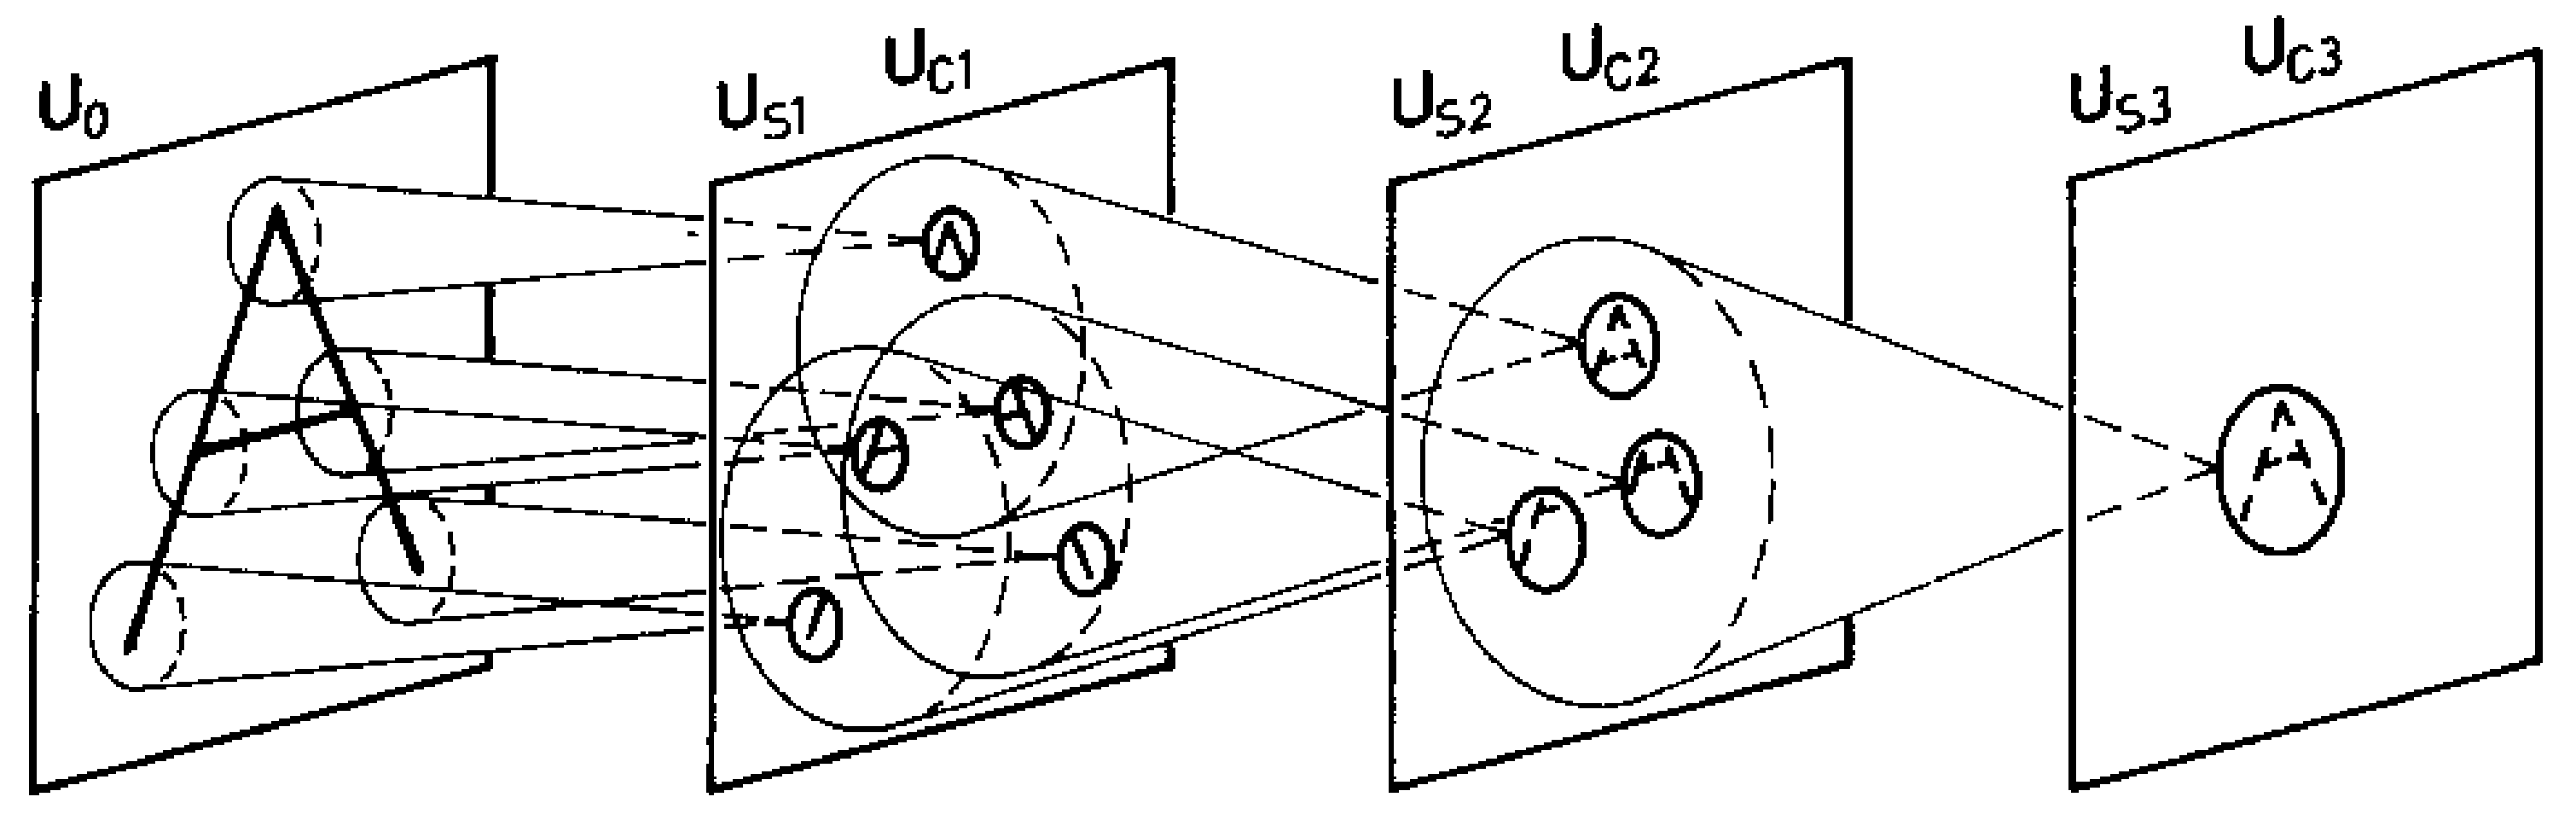
\includegraphics[width=110mm]{img/neocognitron.png}
	\caption{Diagrama del neocognitrón mostrando el flujo de procesamiento de una imagen a través de varias capas. Las capas \(U_{S}\) (simple) y \(U_{C}\) (compleja) procesan la información de forma jerárquica, comenzando con la imagen original \(U_0\) y extrayendo características cada vez más complejas en \(U_{S1}\), \(U_{C1}\), \(U_{S2}\), \(U_{C2}\), \(U_{S3}\) y \(U_{C3}\).}
\end{figure}

Inspirado en estas observaciones, Kunihiko Fukushima desarrolló el \textbf{neocognitrón} en 1980, una red neuronal que es considerada uno de los precursores de las modernas CNNs \cite{fukushima1980neocognitron}. El neocognitrón fue diseñado para reconocer patrones visuales complejos de manera robusta frente a traslaciones y otras pequeñas distorsiones de la imagen. Esta red consta de múltiples capas que alternan entre capas convolucionales, que detectan características locales y capas que agregan las respuestas de los detectores de características sobre áreas locales (\autoref{fig:neocognitron}). La estructura de esta red capta de manera efectiva la forma en que la corteza visual procesa la información visual, implementando una forma primitiva de invarianza a la traslación y la capacidad de extraer características jerárquicas.

La influencia de la corteza visual y el neocognitrón en el diseño de las CNNs es una muestra de la utilidad de estudios interdisciplinarios entre neurociencia y aprendizaje automático. Estos estudios no solo han facilitado avances tecnológicos en visión artificial sino que también han ofrecido nuevas perspectivas sobre cómo los seres humanos procesamos la información visual, proponiendo un puente entre la inteligencia artificial y la biológica \cite{serre2007feedforward}.


\subsection{Arquitectura de una CNN}

Las CNNs, introducidas por Yann LeCun, supusieron un avance significativo respecto al neocognitrón. Mientras que el neocognitrón sentó las bases al proponer una arquitectura inspirada en el procesamiento visual del cerebro, LeCun implementó un método de entrenamiento supervisado utilizando retropropagación, lo que permitió mejorar notablemente el rendimiento y la capacidad de generalización de las redes neuronales \cite{lecun1998gradient}. Además, LeCun sentó las bases de la arquitectura de CNNs, optimizando la eficiencia y escalabilidad de los modelos, incorporando capas como las capas convolucionales y de muestreo \cite{lecun1989backpropagation}.

\begin{figure}
% DEEP CONVOLUTIONAL NEURAL NETWORK
\centering
\begin{tikzpicture}[x=1.3cm,y=0.8cm]
	\large
	\message{^^JDeep convolution neural network}
	\readlist\Nnod{5,5,4,3,2,4,4,3} % array of number of nodes per layer
	\def\NC{6} % number of convolutional layers
	\def\nstyle{int(\lay<\Nnodlen?(\lay<\NC?min(2,\lay):3):4)} % map layer number on 1, 2, or 3
	\tikzset{ % node styles, numbered for easy mapping with \nstyle
		node 1/.style={node in},
		node 2/.style={node convol},
		node 3/.style={node hidden},
		node 4/.style={node out},
	}
	
	% TRAPEZIA
	\draw[myorange!40,fill=myorange,fill opacity=0.02,rounded corners=2]
	%(1.6,-2.5) rectangle (4.4,2.5);
	(1.6,-2.7) --++ (0,5.4) --++ (3.8,-1.9) --++ (0,-1.6) -- cycle;
	\draw[myblue!40,fill=myblue,fill opacity=0.02,rounded corners=2]
	(5.6,-2.0) rectangle++ (1.8,4.0);
	\node[font=\small,right=19,above=10,align=center,myorange!60!black] at (3.1,1.8) {Bloques\\[-0.2em]convolucionales};
	\node[font=\small,above=10,align=center,myblue!60!black] at (6.5,1.9) {Capas ocultas\\[-0.2em]totalmente conectadas};
	
	\message{^^J  Layer}
	\foreachitem \N \in \Nnod{ % loop over layers
		\def\lay{\Ncnt} % alias of index of current layer
		\pgfmathsetmacro\prev{int(\Ncnt-1)} % number of previous layer
		%\pgfmathsetmacro\Nprev{\Nnod[\prev]} % array of number of nodes in previous layer
		\message{\lay,}
		\foreach \i [evaluate={\y=\N/2-\i+0.5; \x=\lay; \n=\nstyle;}] in {1,...,\N}{ % loop over nodes
			%\message{^^J  Layer \lay, node \i}
			
			% NODES
			\node[node \n,outer sep=0.6] (N\lay-\i) at (\x,\y) {};
			
			% CONNECTIONS
			\ifnum\lay>1 % connect to previous layer
			\ifnum\lay<\NC % convolutional layers
			\foreach \j [evaluate={\jprev=int(\i-\j); \cconv=int(\Nnod[\prev]>\N); \ctwo=(\cconv&&\j>0);
				\c=int((\jprev<1||\jprev>\Nnod[\prev]||\ctwo)?0:1);}]
			in {-1,0,1}{
				\ifnum\c=1
				\ifnum\cconv=0
				\draw[connect,white,line width=1.2] (N\prev-\jprev) -- (N\lay-\i);
				\fi
				\draw[connect] (N\prev-\jprev) -- (N\lay-\i);
				\fi
			}
			
			\else % fully connected layers
			\foreach \j in {1,...,\Nnod[\prev]}{ % loop over nodes in previous layer
				\draw[connect,white,line width=1.2] (N\prev-\j) -- (N\lay-\i);
				\draw[connect] (N\prev-\j) -- (N\lay-\i);
			}
			\fi
			\fi % else: nothing to connect first layer
			
		}
	}
	
	% LABELS
	\node[font=\small,above=3,align=center,mygreen!60!black] at (N1-1.90) {Capa de\\[-0.2em]entrada};
	\node[font=\small, above=0,align=center,myred!60!black] at (N\Nnodlen-1.90) {Capa de\\[-0.2em]salida};
	
\end{tikzpicture}
\caption{Arquitectura de una CNN. Muestra la secuencia de capas en la red, iniciando con la capa de entrada, seguida por múltiples bloques convolucionales (resaltados en naranja), continuando con capas ocultas totalmente conectadas (resaltadas en azul) y finalmente la capa de salida. }
\end{figure}

Una CNN típicamente consiste en una secuencia de capas que transforman la entrada de imagen bruta en representaciones cada vez más abstractas y útiles para la tarea en cuestión. Cada tipo de capa dentro de una CNN tiene un propósito específico y contribuye de manera distinta al proceso de aprendizaje. Generalmente, las distintas capas de una CNN suelen agruparse para cumplir distintas funciones. Las principales agrupaciones que componen una CNN son:

\begin{itemize}
	\item \textbf{Capa de entrada}: Es la primera capa de la red, donde se introduce la imagen original o preprocesada. Su función principal es preparar y escalar la imagen para las operaciones de las capas siguientes.
	
	\item \textbf{Bloques convolucionales}: Estos bloques contienen una o más capas convolucionales seguidas frecuentemente por capas de normalización y funciones de activación. Cada capa convolucional aplica diferentes filtros a la entrada para crear mapas de características que resalten aspectos específicos de la imagen. Estos bloques suelen ir consecutivos intercalando capas de muestreo. 
	
	\item \textbf{Capas totalmente conectadas}: Después de varias capas convolucionales y de muestreo, la información en forma de matrices y tensores se aplana en vectores y se pasa a través de capas FC. Estas capas integran la información aprendida por las capas anteriores para realizar la clasificación final.
	
	\item \textbf{Capa de salida}: La última capa de una CNN, donde se obtiene el resultado final. En tareas de clasificación, esta capa suele usar una función de activación como la Softmax para asignar probabilidades a las distintas clases posibles.
\end{itemize}

A continuación, vamos a explorar las diferentes capas que componen estos bloques y cómo trabajan juntas para detectar y aprender patrones importantes en los datos.

\subsubsection{Capa convolucional}

La \textbf{capa convolucional} es el bloque de construcción fundamental de una CNN. Utiliza un conjunto de filtros que se aplican a la entrada mediante el operador de \textbf{convolución discreta}. Cada filtro detecta características específicas en una región local de la entrada. El operador de convolución discreta se puede expresar como:
\begin{equation}
	S(i, j) = (I \ast K)(i, j) = \sum_m \sum_n I(m, n) K(i-m, j-n),
\end{equation}
donde $m,n$ son las coordenadas en la imagen o matriz de entrada \(I\) de la región a convolucionar, $i,j$ son las coordenadas del centro del \textbf{kernel} o \textbf{filtro} \(K\) y \(S\) es la matriz de salida o \textbf{mapa de características}. La convolución discreta es un \textbf{operador lineal}, lo que implica que satisface propiedades como la \textbf{conmutatividad}, \textbf{asociatividad} y \textbf{distributividad}.

Estos filtros se desplazan sobre toda la superficie de la entrada, generando un mapa de características que resume la presencia de las particularidades de dicha entrada.

\usetikzlibrary{positioning, calc, decorations.pathreplacing}
\begin{figure}[H]
	\centering
\begin{tikzpicture}[
	2d-arr/.style={matrix of nodes, row sep=-\pgflinewidth, column sep=-\pgflinewidth, nodes={draw, text height=1.0ex, text depth=0.25ex}}
	]
	
	\matrix (mtr) [2d-arr] {
		0 & 1 & 1 & |[fill=orange!30]| 1 & |[fill=orange!30]| 0 & |[fill=orange!30]| 0 & 0\\
		0 & 0 & 1 & |[fill=orange!30]| 1 & |[fill=orange!30]| 1 & |[fill=orange!30]| 0 & 0\\
		0 & 0 & 0 & |[fill=orange!30]| 1 & |[fill=orange!30]| 1 & |[fill=orange!30]| 1 & 0\\
		0 & 0 & 0 & 1 & 1 & 0 & 0\\
		0 & 0 & 1 & 1 & 0 & 0 & 0\\
		0 & 1 & 1 & 0 & 0 & 0 & 0\\
		1 & 1 & 0 & 0 & 0 & 0 & 0\\
	};
	
	\node[below=of mtr-5-4] {$\mathbf I$};
	
	\node[right=0.2em of mtr] (str) {$*$};
	
	\matrix (K) [2d-arr, right=0.2em of str, nodes={draw, fill=teal!30}] {
		1 & 0 & 1 \\
		0 & 1 & 0 \\
		1 & 0 & 1 \\
	};
	\node[below=of K-3-2] {$\mathbf K$};
	
	\node[right=0.2em of K] (eq) {$=$};
	
	\matrix (ret) [2d-arr, right=0.2em of eq] {
		1 & 4 & 3 & |[fill=blue!80!black!30]| 4 & 1\\
		1 & 2 & 4 & 3 & 3\\
		1 & 2 & 3 & 4 & 1\\
		1 & 3 & 3 & 1 & 1\\
		3 & 3 & 1 & 1 & 0\\
	};
	\node[below=of ret-4-3] {$\mathbf{I * K}$};
	
	\draw[dashed, teal] (mtr-1-6.north east) -- (K-1-1.north west);
	\draw[dashed, teal] (mtr-3-6.south east) -- (K-3-1.south west);
	
	\draw[dashed, blue!80!black] (K-1-3.north east) -- (ret-1-4.north west);
	\draw[dashed, blue!80!black] (K-3-3.south east) -- (ret-1-4.south west);
	
	\foreach \i in {1,2,3} {
		\foreach \j in {4,5,6} {
			\node[font=\tiny, scale=0.6, shift={(-1.2ex,-2ex)}] at (mtr-\i-\j) {$\times \pgfmathparse{int(mod(\i+\j,2))}\pgfmathresult$};
		}
	}
	
\end{tikzpicture}
\caption{Ejemplo de convolución discreta. La matriz de entrada $\mathbf{I}$ se muestra con un segmento resaltado en naranja, mostrando la región afectada por el filtro $\mathbf{K}$, en color verde. La matriz resultante $\mathbf{I * K}$ destaca los valores resultantes de la convolución, con el resultado de la convolución en dicha región en azul.}
\end{figure}

Además de las propiedades del operador de convolución, las capas convolucionales muestran varias propiedades más que las hacen especialmente adecuadas para tareas de procesamiento de imágenes y visión artificial. Entre estas propiedades destacan:

\begin{itemize}
	\item \textbf{Conectividad local:}
	Cada neurona en una capa convolucional está conectada solo a un pequeño número de neuronas cercanas en la capa anterior. Esta estructura imita la manera en que los campos receptivos en el sistema visual humano se organizan, concentrándose en pequeñas regiones del espacio visual. La conectividad local permite a la red detectar características locales de la entrada sin la influencia de la estructura global, reduciendo la complejidad y el número total de parámetros necesarios.
	
	\item \textbf{Compartición de parámetros:}
	En una CNN, el mismo filtro se utiliza para cada posición de la entrada, a diferencia de una red neuronal completamente conectada donde cada peso es único para cada conexión. Esta compartición de parámetros permite que la red sea más eficiente en términos de memoria y computación. Además, también implica que las características aprendidas por un filtro son útiles en toda la imagen, lo que mejora la eficiencia del aprendizaje y ayuda a la red a generalizar mejor.
	
	\item \textbf{Equivarianza frente a traslaciones:}
	Debido al uso de la misma función de convolución a lo largo de toda la entrada, las CNNs son naturalmente equivariantes a las traslaciones. Esto significa que si la entrada se traslada, las características detectadas por la red también se trasladarán de manera correspondiente. Esta propiedad es particularmente interesante en tareas de visión artificial, donde la relevancia de una característica no suele depender de su posición específica en el espacio de entrada.
\end{itemize}

Los hiperparámetros de \textbf{paso} o \textbf{\textit{stride}}, y \textbf{relleno} o \textbf{\textit{padding}} son especialmente relevantes en la manipulación dimensional durante la convolución en CNNs. El \textit{stride} define el paso con el que el filtro se desplaza sobre la imagen o mapa de características, afectando la reducción dimensional del mapa resultante y permitiendo la captura de características a diversas escalas. Por otro lado, el \textit{padding} consiste en añadir píxeles artificiales alrededor de la imagen de entrada, lo que permite que el filtro acceda completamente a los bordes y mantiene el tamaño del volumen de salida, preservando la información en los bordes cruciales para la interpretación completa de la imagen.

\begin{figure}[H]
	\centering
	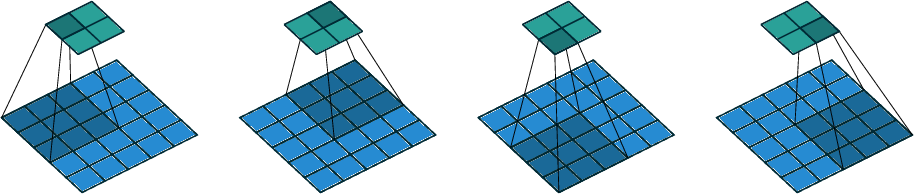
\includegraphics[width=100mm]{img/stride.png}
	\caption{Convolución de un filtro de 3x3 sobre una entrada de 5x5. La operación se realiza utilizando \textit{strides} de 2x2 y sin agregar relleno (\textit{padding} = 0), lo que resulta en una matriz de salida más pequeña y eficientemente espaciada. Fuente \cite{Dumoulin2016AGT}.}
\end{figure}
\begin{figure}[H]
	\centering
	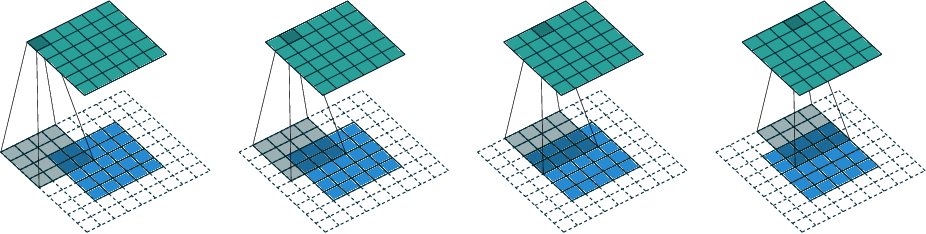
\includegraphics[width=100mm]{img/padding.png}
	\caption{Convolución de un filtro de 3x3 sobre una entrada de 5x5. Se emplea un relleno de 2 unidades y pasos unitarios (\textit{stride} = 1), asegurando que la matriz de salida aumente las dimensiones de la matriz de entrada, al expandir el borde de la imagen original. Fuente \cite{Dumoulin2016AGT}.}
\end{figure}

La elección de dichos hiperparámetros influye directamente en las dimensiones del mapa de características de salida, cuya altura \(H_{\text{out}}\) y anchura \(W_{\text{out}}\) vienen dadas de la siguiente manera:
\[
H_{\text{out}} = \left\lfloor \frac{H_{\text{in}} + 2P - H_{\text{f}}}{S} + 1 \right\rfloor, \quad
W_{\text{out}} = \left\lfloor \frac{W_{\text{in}} + 2P - W_{\text{f}}}{S} + 1 \right\rfloor,
\]
donde \(H_{\text{in}}\) y \(W_{\text{in}}\) son las dimensiones de entrada, \(H_{\text{f}}\) y \(W_{\text{f}}\) son las del filtro, \(P\) es el \textit{padding}, \(S\) es el \textit{stride} y $\lfloor \cdot \rfloor$ denota la función suelo. La profundidad del mapa de salida, \(D_{\text{out}}\), está determinada por el número de filtros aplicados, donde \( D_{\text{out}} = \text{número de filtros} \).

Estas convoluciones, aunque predominantemente asociadas con dimensiones bidimensionales, pueden extenderse a contextos tridimensionales (3D) donde se aplican filtros 3D sobre varios canales al mismo tiempo. Por ejemplo, un filtro de tamaño $1 \times 1 \times 1$ puede transformar linealmente los mapas de características en cada ubicación del volumen de entrada. Las dimensiones de salida se mantienen como:
\[
H_{\text{out}} = H_{\text{in}}, \quad W_{\text{out}} = W_{\text{in}}, \quad D_{\text{out}} = \text{número de filtros}.
\]
Nótese que estas convoluciones son importantes para ajustar la dimensionalidad de los canales dentro de redes profundas, pues con una sola \textbf{convolución $1 \times 1$} podemos colapsar todos los canales de entrada en uno solo. Esto supone una reducción efectiva de parámetros y de la complejidad computacional en datos tridimensionales.

Otro tipo de convoluciones que surge en este contexto son las \textbf{convoluciones en profundidad} o \textbf{\textit{depthwise convolutions}}. En ellas, cada filtro se aplica de manera independiente a cada canal del volumen de entrada, permitiendo un procesamiento separado de las dimensiones espaciales y de profundidad. La fórmula para las dimensiones de salida se mantiene, pero esta vez manteniendo el número de canales:
\[
H_{\text{out}} = \left\lfloor \frac{H_{\text{in}} + 2P - H_{\text{f}}}{S} + 1 \right\rfloor, \quad W_{\text{out}} = \left\lfloor \frac{W_{\text{in}} + 2P - W_{\text{f}}}{S} + 1 \right\rfloor, \quad D_{\text{out}} = D_{\text{in}}.
\]
Estas convoluciones son eficaces para optimizar el rendimiento computacional en aplicaciones donde el manejo eficiente de los recursos es esencial.

\subsubsection{Capa de muestreo}

Las capas de \textbf{muestreo}, conocidas generalmente como capas de \textbf{\textit{pooling}}, buscan reducir la dimensionalidad espacial de los mapas de características, lo que permite disminuir la cantidad de parámetros y de cómputo en la red al mismo tiempo que se mantiene la información más relevante. Las capas de \textit{pooling} más comunes son las de \textbf{máximo} o \textbf{\textit{max pooling}}, y las de \textbf{promedio} o \textbf{\textit{average pooling}}. El \textit{max pooling} toma la mayor activación en la ventana del filtro como:
\begin{equation}
	P(i, j) = \max_{m, n \in W} I(i+m, j+n),
\end{equation}
donde \(W\) es la ventana del filtro de \textbf{pooling}. Esta operación ayuda a hacer la representación obtenida invariante a pequeñas traslaciones y distorsiones. Por otro lado, el \textit{average pooling} calcula el promedio de las activaciones dentro de la ventana del filtro, proporcionando una representación que suaviza las características de entrada:
\begin{equation}
	P(i, j) = \frac{1}{|W|} \sum_{a, b \in W} I(i+a, j+b),
\end{equation}
donde \(|W|\) es el número de elementos en la ventana del filtro. Ambas técnicas de pooling tienen sus aplicaciones específicas dependiendo de la naturaleza del problema y de la arquitectura de la red. Mientras que el \textit{max pooling} es generalmente preferido para tareas relacionadas con la detección de características debido a su capacidad para preservar las activaciones más fuertes, el \textit{average pooling} puede ser más adecuado para tareas donde la uniformidad de las características es más importante \cite{krizhevsky2012imagenet}.

\newcommand{\matrixA}{%     
	\setlength{\tabcolsep}{0pt}
	\begin{NiceTabular}{*{4}{c}}[hvlines,rules/width=2pt, cell-space-limits=1.0ex,columns-width=4ex]
		\CodeBefore % color the blocks
		\rectanglecolor{blue!15}{1-1}{2-2}
		\rectanglecolor{green!15}{3-1}{4-2}
		\rectanglecolor{orange!25}{1-3}{2-4}
		\rectanglecolor{red!15}{3-3}{4-4}
		\Body   
		\RowStyle[nb-rows=4]{\bfseries} % make all bold
		8&7&5&3\\
		12&9&5&7\\
		13&2&10&3\\
		9&4&5&14\\      
	\end{NiceTabular}
}

\newcommand{\matrixB}{% 
	\setlength{\tabcolsep}{0pt}
	\begin{NiceTabular}{*{2}{c}}[hvlines,rules/width=1.6pt,cell-space-limits=1.0ex,columns-width=4ex]
		\CodeBefore % color the cells
		\cellcolor{blue!15}{1-1}
		\cellcolor{orange!15}{1-2}
		\cellcolor{green!15}{2-1}
		\cellcolor{red!15}{2-2}
		\Body   
		\RowStyle[nb-rows=2]{\bfseries} % make all bold
		12&7\\
		13&14\\     
	\end{NiceTabular}
}

\newcommand{\matrixC}{% 
	\setlength{\tabcolsep}{0pt}
	\begin{NiceTabular}{*{2}{c}}[hvlines,rules/width=1.6pt,cell-space-limits=1.0ex, columns-width=4ex]
		\CodeBefore % color the cells
		\cellcolor{blue!15}{1-1}
		\cellcolor{orange!15}{1-2}
		\cellcolor{green!15}{2-1}
		\cellcolor{red!15}{2-2}
		\Body   
		\RowStyle[nb-rows=2]{\bfseries} % make all bold
		9&5\\
		7&8\\       
	\end{NiceTabular}
}

\begin{figure}
	\centering
\begin{tikzpicture}
	% layout the matrices
	\node (matA) {\matrixA};
	\node[ above right = -30pt and 150pt of matA, scale=1.2, anchor = south west] (matB) {\matrixB};
	\node[ below right = -20pt and 150pt of matA, scale=1.2, anchor =north  west] (matC) {\matrixC};
	% a large parenthesis
	\node (paren) [right = 120pt of matA] {$\left(\rule{0pt}{100pt}\right.$};
	% the arrow
	\draw[-latex,ultra thick,  shorten >=3mm, shorten <=2mm,] (matA.east) -- (paren.center)  node[midway,above, text width=3cm,     font= \bfseries, text centered] {2x2 pooling, stride 2};    
	% add the labels
	\node[above =  -3pt of matB.north,font=\bfseries]{Max pooling};
	\node[above =  -3pt of matC.north,font=\bfseries]{Average pooling};
\end{tikzpicture}  
\caption{Comparación de técnicas de \textit{pooling}. Arriba, \textit{max pooling} y abajo, \textit{average pooling}, ambas con un filtro de 2x2 y \textit{stride} de 2, mostrando la transformación de la matriz original.}
\end{figure}

%La \textbf{normalización} es un paso crucial en muchas CNNs que ayuda a acelerar la convergencia del entrenamiento y reduce la sensibilidad a la inicialización de los parámetros de la red. La normalización por lotes es una técnica común que normaliza las salidas de la capa anterior por mini-batch, ajustando y escalando las activaciones para tener una media cero y una varianza unitaria.
%
%\subsubsection{Capa totalmente conectada}
%
%Las capas FC en las CNNs desempeñan un papel importante al transformar las características extraídas por las capas convolucionales y de \textit{pooling} en predicciones finales. Al final de la arquitectura de la red, estas capas funcionan como clasificadores, interpretando las características y tomando decisiones basadas en ellas para clasificar la entrada en diferentes categorías. Además, en la \textbf{transferencia de aprendizaje} o \textbf{\textit{transfer learning}}, estas capas pueden ser reemplazadas o ajustadas para adaptarse a nuevas tareas, mientras que las capas convolucionales anteriores se utilizan para aprovechar las características genéricas aprendidas.

\subsection{Modelos y estado del arte en CNNs}

Desde su concepción, las arquitecturas de CNNs han experimentado una evolución significativa, marcada por una serie de innovaciones clave que han mejorado su rendimiento y eficiencia. Como vimos anteriormente, la historia de las CNNs comenzó con el neocognitrón de Fukushima en los años 80 \cite{fukushima1980neocognitron}, un modelo pionero que introdujo el concepto de capas convolucionales y de pooling. Posteriormente, la introducción de LeNet-5 por LeCun et al. en los años 90 \cite{lecun1998gradient} demostró la eficacia de las CNNs en tareas de reconocimiento de dígitos y documentos, mostrando que este tipo de arquitecturas podían aprender a resolver problemas de aprendizaje supervisado. Posteriormente AlexNet, desarrollada por Krizhevsky et al. en 2012 \cite{krizhevsky2012imagenet}, revolucionó el campo del aprendizaje profundo, utilizando técnicas como paralización del entrenamiento, profundización de la red, ReLU y dropout para ganar el desafío de ImageNet con una reducción drástica en la tasa de error. A partir de ahí, surgieron modelos más sofisticados como VGG \cite{simonyan2014very}, GoogLeNet con su módulo Inception \cite{szegedy2015going}, o ResNet, que introdujo las conexiones residuales permitiendo entrenar redes mucho más profundas \cite{he2016deep}. Cada una de estas arquitecturas ha contribuido a comprender mejor cómo diseñar redes eficientes para procesar y aprender de imágenes a gran escala. En la actualidad, modelos más recientes como DenseNet, que conecta cada capa directamente con todas las anteriores \cite{huang2017densely}, y EfficientNet, que escala de manera uniforme todas las dimensiones de la red \cite{tan2019efficientnet}, continúan empujando los límites de lo que las CNNs pueden lograr, optimizando el rendimiento y la eficiencia para aplicaciones en tiempo real y en dispositivos con recursos limitados.

\subsubsection{ResNet}

Las \textbf{Redes Neuronales Residuales} (ResNet) introducidas por He et al. en 2015, supusieron un avance significativo en la arquitectura de redes profundas para el reconocimiento de imágenes. A diferencia de sus predecesores como AlexNet y VGG, ResNet aborda el problema del desvanecimiento del gradiente que suele presentarse en redes muy profundas mediante la introducción de una conexión de identidad que salta una o más capas.

La clave de la arquitectura de ResNet es el \textbf{bloque residual}, que incorpora una \textbf{conexión residual} directamente conectando la entrada del bloque a su salida, lo que permite que la señal se propague directamente a través de la red. El bloque residual se puede expresar como:
\begin{equation}
	H(\mathbf{x}_l) = \mathcal{F}(\mathbf{x}_l, \{W_i\}) + \mathbf{x}_l
\end{equation}
donde \(\mathbf{x}_l\) y \(H(\mathbf{x}_l)\) son la entrada y la salida del $l$-ésimo bloque residual respectivamente, \(\mathcal{F}\) representa las capas intermedias de la red y \(\{W_i\}\) denota el conjunto de pesos de estas capas.

\begin{figure}
	\centering
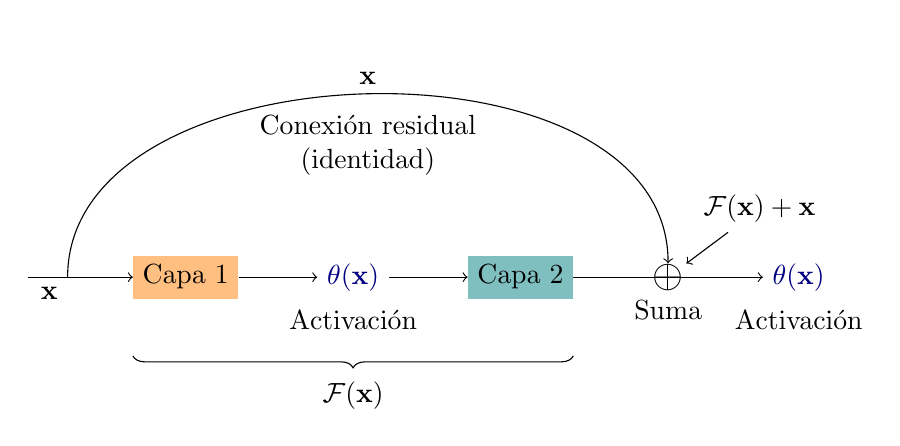
\begin{tikzpicture}
	
	\node[fill=orange!50] (l1) {Capa 1};
	\node[blue!50!black, right=of l1, label={below:Activación}] (act1) {$\theta(\mathbf{x})$};
	\node[fill=teal!50, right=of act1] (l2) {Capa 2};
	\node[right=of l2, font=\Large, label={below:Suma}, inner sep=0, pin={60:$\mathcal F(\mathbf{x}) + \mathbf{x}$}] (add) {$\oplus$};
	\node[blue!50!black, right=of add, label={below:Activación}] (act2) {$\theta(\mathbf{x})$};
	
	\draw[->] (l1) -- (act1);
	\draw[->] (act1) -- (l2);
	\draw[<-] (l1) -- ++(-2,0) node[below, pos=0.8] {$\mathbf{x}$};
	\draw[->] (l2) -- (act2) node[above, pos=0.8] {};
	\draw[->] ($(l1)-(1.5,0)$) to[out=90, in=90] node[below=1ex, midway, align=center] {Conexión residual\\(identidad)} node[above, midway] {$\mathbf{x}$} (add);
	\draw[decorate, decoration={brace, amplitude=1ex, raise=1cm}] (l2.east) -- node[midway, below=1.2cm] {$\mathcal F(\mathbf{x})$} (l1.west);
	
\end{tikzpicture}
\caption{Diagrama de una conexión residual. La entrada $\mathbf{x}$ pasa a través de la Capa 1 y una función de activación, fluyendo luego hacia la Capa 2. Paralelamente, $\mathbf{x}$ se suma directamente al final de la Capa 2 mediante una conexión residual. }
\end{figure}

A diferencia de AlexNet, que tiene 8 capas, y VGG, que tiene 16 o 19 capas, ResNet se diseñó con capacidades mucho más profundas, con versiones que van desde 18 hasta 152 capas. Lo revolucionario de ResNet no es simplemente añadir más capas, sino su habilidad para entrenar redes muy profundas sin sufrir desvanecimiento del rendimiento gracias a sus conexiones residuales. Estas conexiones ayudan a preservar el gradiente a lo largo del proceso de aprendizaje, lo que permite entrenar redes que son significativamente más profundas que las posibles anteriormente.

El diseño del bloque residual permite que ResNet no solo evite el problema del desvanecimiento del gradiente sino que también mejore la eficiencia del entrenamiento. Los experimentos demuestran que las redes con bloques residuales superan a las arquitecturas convencionales en varias métricas importantes, como la precisión en conjuntos de datos de imágenes de gran escala, incluido ImageNet.

\subsubsection{DenseNet}

Las \textbf{Redes Convolucionales Densamente Conectadas} (DenseNet) propuestas por Huang et al. en 2017, representan otra evolución significativa en el diseño de redes neuronales profundas. DenseNet mejora la idea de conexiones de salto de ResNet mediante la integración de cada capa directamente con todas las capas posteriores de una manera densamente conectada.

La principal innovación de DenseNet es su estructura de \textbf{conexiones densas}, donde cada capa recibe como entrada todas las salidas de las capas anteriores, concatenando estas salidas. Esto se formula como sigue:
\begin{equation}
	\mathbf{x}_l = H_{l}([\mathbf{x}_0, \mathbf{x}_1, \dots, \mathbf{x}_{l-1}])
\end{equation}
donde \(\mathbf{x}_l\) es la salida de la capa \(l\), \([ \cdot ]\) denota la operación de concatenación y \(H_l\) es una función que representa las operaciones dentro de la capa \(l\), normalmente compuesta por operaciones de \textit{Batch Normalization}, activación ReLU, y convolución.

\begin{figure}
	\label{key}
	\centering
	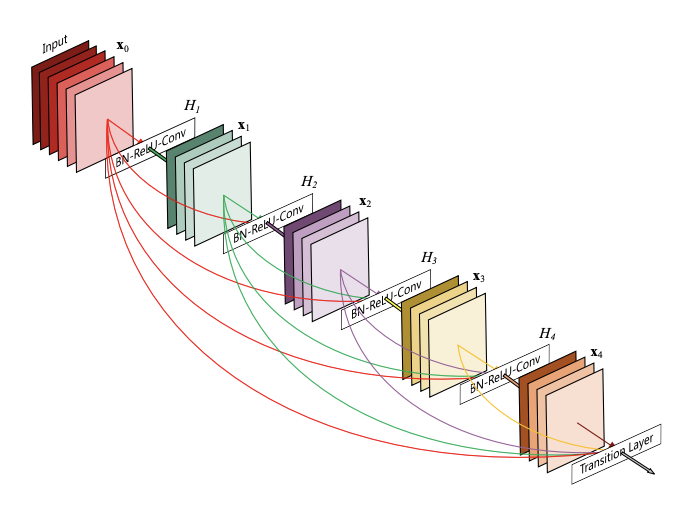
\includegraphics[width=100mm]{img/densenet.png}
	\caption{Arquitectura de DenseNet. La figura ilustra la configuración de la red DenseNet, mostrando cómo las capas están conectadas entre sí, donde cada capa recibe como entrada todas las salidas de las capas anteriores. Fuente \cite{huang2017densely}.}
\end{figure}

Aunque tanto ResNet como DenseNet utilizan conexiones que saltan capas, DenseNet ofrece una mejora en la eficiencia y la efectividad del entrenamiento al promover la reutilización de características de manera más intensiva. Mientras que las conexiones de salto en ResNet suman entradas, en DenseNet la información fluye a través de la red mediante la concatenación de características, lo que resulta en una mejora del flujo de información y gradientes a través de la red, reduciendo así el problema del desvanecimiento del gradiente de manera más efectiva.

DenseNet ha demostrado ser particularmente eficaz en conjuntos de datos como ImageNet y en aplicaciones donde la conservación de la información a lo largo de la red es crítica. Además, DenseNet tiende a ser más eficiente en términos de parámetros que ResNet debido a su capacidad para reutilizar características, lo que permite la construcción de redes profundas que son tanto compactas como potentes.

\subsubsection{EfficientNet}

\textbf{EfficientNet}, introducido por Tan y Le en 2019, es un ejemplo de cómo se puede mejorar la eficiencia y la efectividad de las redes neuronales mediante una cuidadosa optimización de sus dimensiones. Esta método de diseñar arquitecturas destaca por utilizar un enfoque sistemático para escalar el ancho, la profundidad y la resolución de las redes.

\begin{figure}
	\centering
	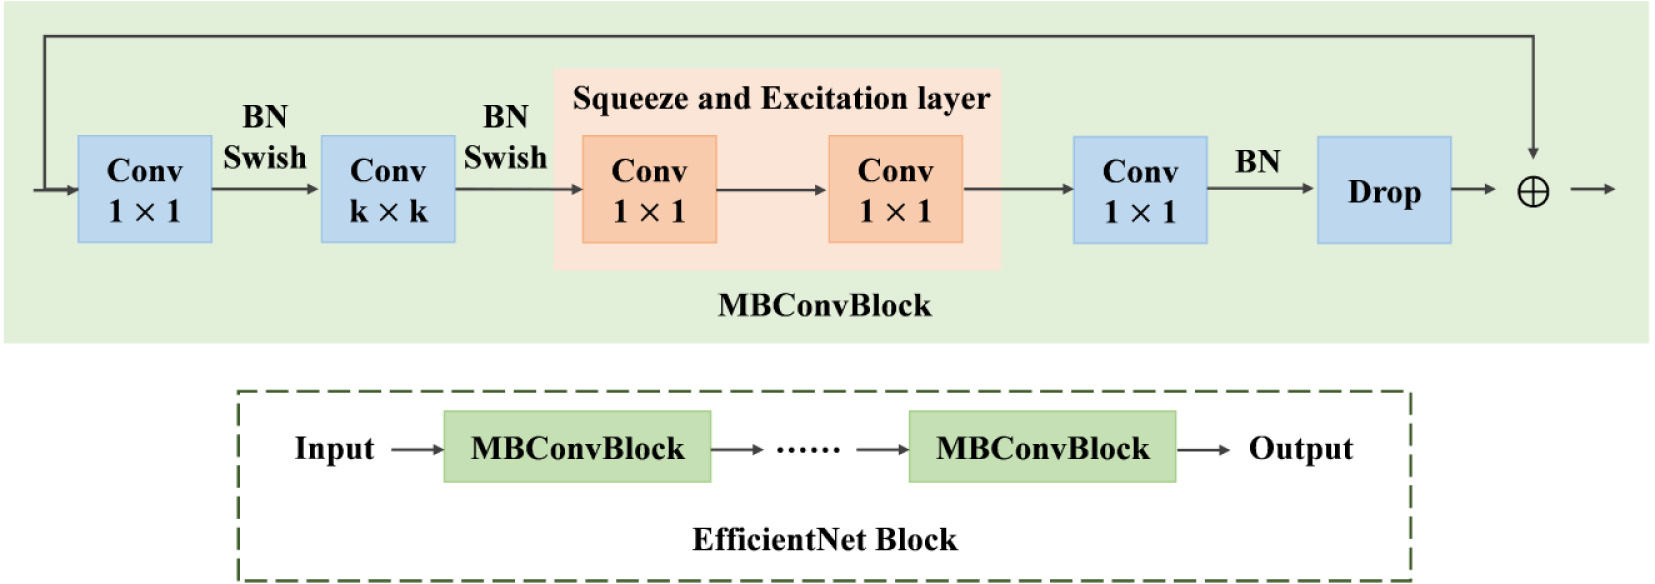
\includegraphics[width=140mm]{img/mbconv.jpg}
	\caption{Estructura de un bloque MBConv, la unidad básica en la arquitectura de EfficientNet.  Incluye capas convolucionales con activaciones Swish y normalización por lotes, intercaladas con capas SE para una afinación eficiente de características. La secuencia de procesamiento termina en una capa de \textit{dropout} antes de la salida final. Fuente \cite{TANG2024105605}.}
\end{figure}

Lo innovador de EfficientNet es su metodología de escalado compuesto, que escala uniformemente todas las dimensiones de la red (profundidad, ancho y resolución de la imagen) con un conjunto fijo de coeficientes de escalado. La fórmula de escalado se representa como:
\begin{equation}
	\text{profundidad}: d = \alpha^\phi, \quad \text{anchura}: w = \beta^\phi, \quad \text{resolución}: r = \gamma^\phi,
\end{equation}
tal que 
\[
\alpha \cdot \beta^2 \cdot \gamma^2 \approx 2, \quad \alpha \geq 1, \quad \beta \geq 1, \quad \gamma \geq 1,
\]

donde \(\phi\) es un coeficiente que determina la cantidad de recursos disponibles para el escalado, y \(\alpha\), \(\beta\), \(\gamma\) son constantes que definen cómo deben escalar la profundidad, el ancho y la resolución, respectivamente, para lograr un equilibrio óptimo entre precisión y eficiencia.

\textbf{EfficientNet-B0} es el modelo base en la familia de modelos \textbf{EfficientNet}, que se caracteriza por aplicar un escalado uniforme a una arquitectura optimizada mediante búsqueda de arquitectura neuronal (NAS). La arquitectura inicia con una capa convolucional de \(3 \times 3\) que maneja la imagen de entrada, aplicando la función de activación Swish y normalización por lotes para preparar las características para las etapas subsiguientes. A continuación, EfficientNet-B0 implementa una serie de \textbf{bloques MBConv}. Cada bloque MBConv sigue un patrón específico:

\begin{enumerate}
	\item \textbf{Expansión:} Primero, una convolución \(1 \times 1\) incrementa el número de canales. Esta técnica de expansión prepara los canales para una manipulación más intensiva, facilitando una rica extracción de características.
	
	\item \textbf{Convolución de profundidad:} Seguidamente, se aplica una convolución en profundidad con un filtro \(3 \times 3\) o \(5 \times 5\). Esta técnica permite la extracción de características locales de manera eficiente, sin el incremento significativo en el número de parámetros que se observaría con convoluciones regulares. La convolución de profundidad provoca una expansión inicial que permite un procesamiento detallado antes de condensar la información nuevamente.
	
	\item \textbf{Capa \textit{Squeeze and Excitation} (SE):} Esta capa sigue a la convolución de profundidad. Funciona primero reduciendo espacialmente cada canal a un valor escalar (\textit{squeeze}), que luego se utiliza para recalibrar los canales (\textit{excitation}) mediante operaciones de reescalado. Este proceso permite al modelo aprender a enfocar dinámicamente su atención en características informativas y suprimir las menos útiles.
	
	\item \textbf{Compresión:} Después de la capa SE, una convolución \(1 \times 1\) reduce el número de canales, consolidando las características importantes, lo cual asegura la eficiencia de la red y prepara la salida para la siguiente etapa del procesamiento.
\end{enumerate}

Las capas de reducción, situadas entre grupos de bloques MBConv, emplean convoluciones con un paso de 2 para reducir las dimensiones espaciales, aumentando el nivel de abstracción y reduciendo la carga computacional en las capas más profundas. Estas capas de transición son cruciales para preparar las características para las etapas de procesamiento subsiguientes.

Finalmente, conexiones residuales se incorporan en cada bloque MBConv para facilitar el entrenamiento de la red al prevenir el desvanecimiento del gradiente. La red culmina con una capa de pooling promedio global que transforma la salida de los bloques MBConv en un vector único por imagen, el cual es procesado por una capa FC para realizar la clasificación final.

Las características clave de EfficientNet-B0, como la función de activación swish y la normalización por lotes después de cada convolución, contribuyen a la estabilidad y la eficiencia del entrenamiento, mejorando la generalización del modelo en aplicaciones de visión por computadora.

A diferencia de ResNet y DenseNet, que principalmente se enfocan en mejorar la profundidad de la red o la densidad de las conexiones, EfficientNet proporciona un marco holístico que ajusta de manera equilibrada todas las dimensiones de la red. Esto no solo mejora el rendimiento sino que también aumenta la eficiencia del modelo, permitiendo que EfficientNet supere a modelos anteriores en precisión con un número significativamente menor de parámetros y una menor cantidad de operaciones de punto flotante (FLOPs).

\begin{figure}
	\centering
	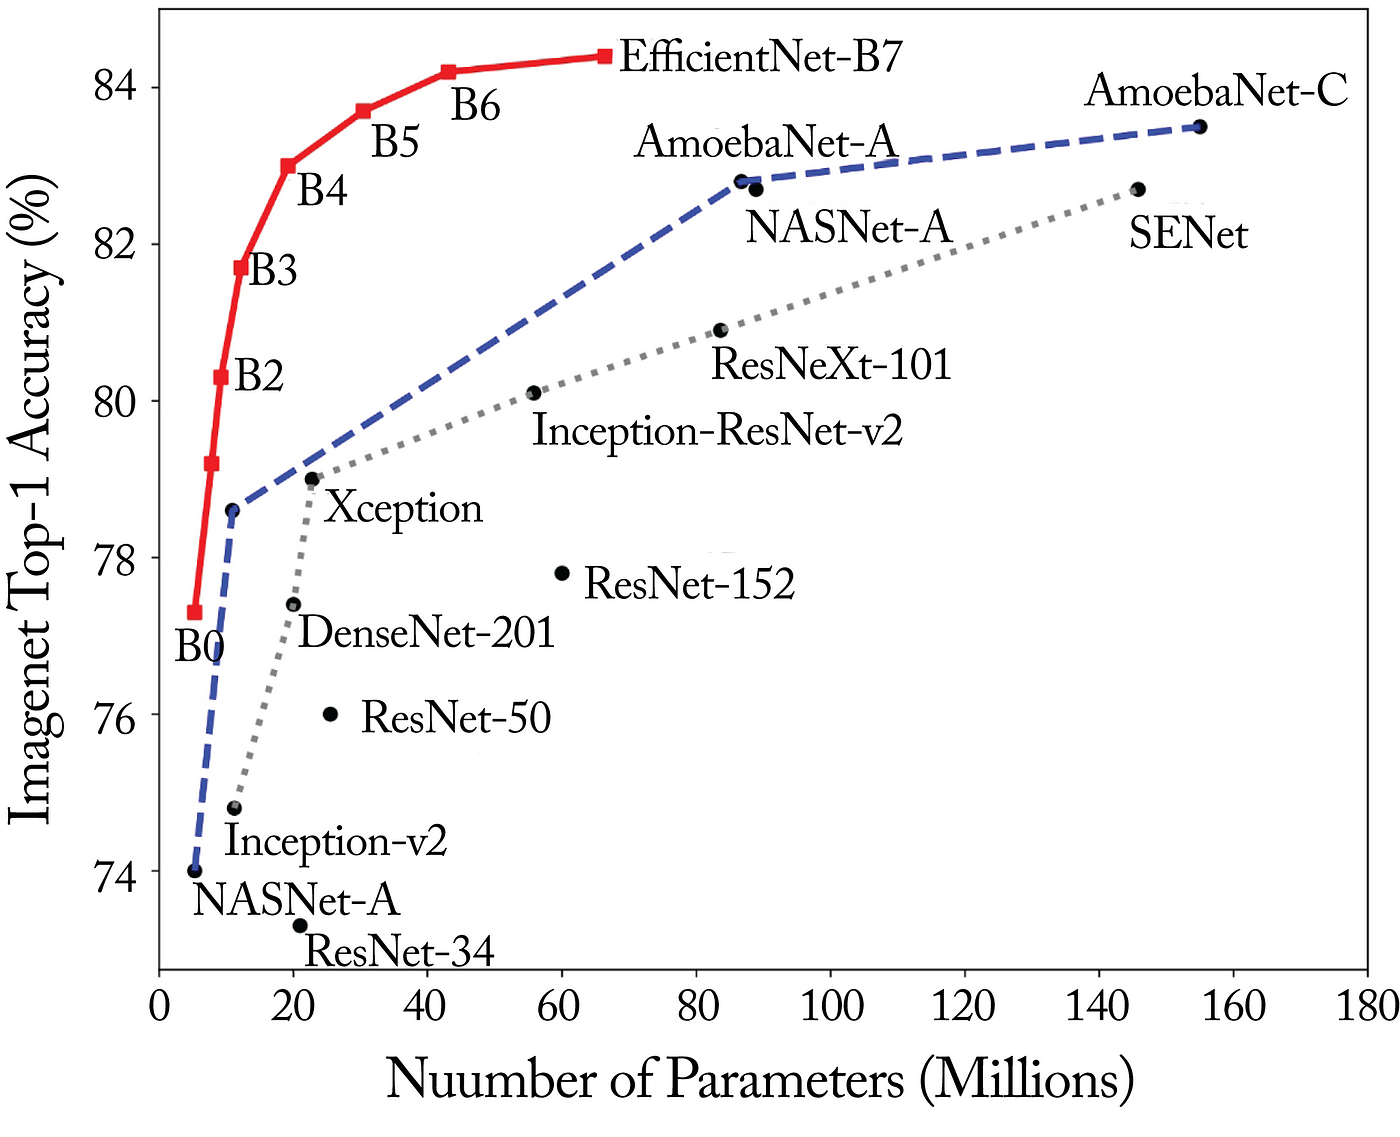
\includegraphics[width=100mm]{img/cnn-sota.png}
	\caption{Comparación de tamaño de modelo y precisión en ImageNet. EfficientNet supera notablemente al resto de modelos de CNNs. En general, EfficientNet muestra una mejora destacable en eficiencia y rendimiento comparado con modelos previos como ResNet-152.}
\end{figure}

En la actualidad, la clasificación de imágenes es considerada por muchos en el campo de la visión artificial como un problema "resuelto", gracias a los avances en las arquitecturas de redes neuronales convolucionales (CNNs). Modelos como ResNet, Inception y EfficientNet han establecido nuevos estándares de precisión en benchmarks como ImageNet, donde las tasas de error se han reducido de manera significativa en comparación con los métodos tradicionales basados en características manuales. Estas arquitecturas avanzadas han demostrado no solo una gran capacidad de generalización sobre grandes conjuntos de datos, sino también una notable robustez frente a variaciones y perturbaciones en las imágenes. Además, la integración de técnicas como el aumento de datos y la \textbf{transferencia de aprendizaje} o \textbf{\textit{transfer learning}}, ha permitido aplicar modelos entrenados en un dominio específico a nuevos conjuntos de datos con poco o ningún ajuste adicional. Este progreso ha transformado la clasificación de imágenes de ser un desafío técnico a una herramienta utilitaria, con aplicaciones en múltiples industrias, desde el reconocimiento automático de contenido en redes sociales hasta sistemas avanzados de asistencia al conductor en vehículos autónomos.

\section{Análisis de datos topológico}

El \textbf{análisis de datos} es una disciplina esencial en la ciencia de datos que se vale de métodos estadísticos, aprendizaje automático y sistemas de procesamiento para transformar grandes cantidades de datos crudos en información útil, crucial para tomar decisiones en diversos campos. Con el desarrollo de esta área, se han integrado técnicas avanzadas como la \textbf{topología algebraica}, que explora propiedades que se mantienen constantes a pesar de las transformaciones físicas de los objetos, enfocándose en aspectos como la continuidad y la conectividad más allá de la forma exacta.

Recordemos que dentro de este contexto, la \textbf{homología} destaca como una herramienta de la topología algebraica diseñada para detectar y analizar características como componentes conexas, agujeros y vacíos en múltiples dimensiones de un espacio. Los conjuntos de datos, que a menudo se presentan como nubes de puntos, representan muestras discretas que podrían sugerir estructuras subyacentes similares a \textbf{variedades topológicas}. Para explorar estas estructuras sin introducir sesgos en cómo se conectan estos puntos, se considera un amplio rango de estructuras en función de la distancia denominadas filtraciones, dando origen a la \textbf{homología persistente}. Esta herramienta no solo identifica características topológicas sino también evalúa su persistencia a lo largo de diversas escalas, lo que ayuda a distinguir entre el ruido y las estructuras significativas.

El \textbf{Análisis de Datos Topológico} (TDA) aprovecha estas técnicas en una metodología avanzada que se centra en desentrañar la estructura subyacente de los datos, basándose en su "forma". Utilizando la homología persistente como su herramienta principal, el TDA ofrece una forma robusta y detallada de identificar las características fundamentales de los datos, permitiendo revelar patrones y relaciones no evidentes mediante métodos tradicionales. Esta metodología se ha aplicado con éxito en varios campos, como la neurociencia para analizar la conectividad cerebral, en genómica para explorar la interacción entre genes, y en ciencia de materiales para estudiar la estructura microscópica de los materiales. Estos casos de uso demuestran cómo el TDA puede proporcionar conocimiento relevante y renovar nuestra comprensión de los sistemas complejos en investigación, ingeniería y análisis social \cite{10.3389/frai.2021.667963}.

El proceso de TDA se organiza en tres fases esenciales que facilitan una comprensión profunda tanto de la topología como de la geometría de los conjuntos de datos:

\begin{enumerate}
	\item \textbf{Preparación de datos}: Inicialmente, se asume que los datos están dispuestos en un espacio métrico, típicamente el espacio euclídeo $\R^N$, utilizando la distancia euclídea como métrica. La elección de esta métrica es crucial, ya que influye directamente en cómo se perciben las distancias y relaciones entre los puntos dentro del conjunto de datos.
	
	\item \textbf{Construcción de filtraciones}: Posteriormente, se desarrolla una serie de complejos simpliciales, estructuras geométricas que se generan al conectar puntos dentro de una distancia determinada. Esta construcción es fundamental para visualizar la evolución de las conexiones entre los puntos conforme se varían los parámetros de escala.
	
	\item \textbf{Extracción de características topológicas}: Finalmente, se emplea la homología persistente para analizar las filtraciones construidas, obteniendo descriptores topológicos que revelan la presencia de características como agujeros y conexiones en diversas dimensiones. Estos descriptores proporcionan una visión detallada de las propiedades topológicas y geométricas de los datos, ayudando a distinguir entre rasgos estructurales significativos y el ruido.
\end{enumerate}

\begin{figure}[H]
	\centering
	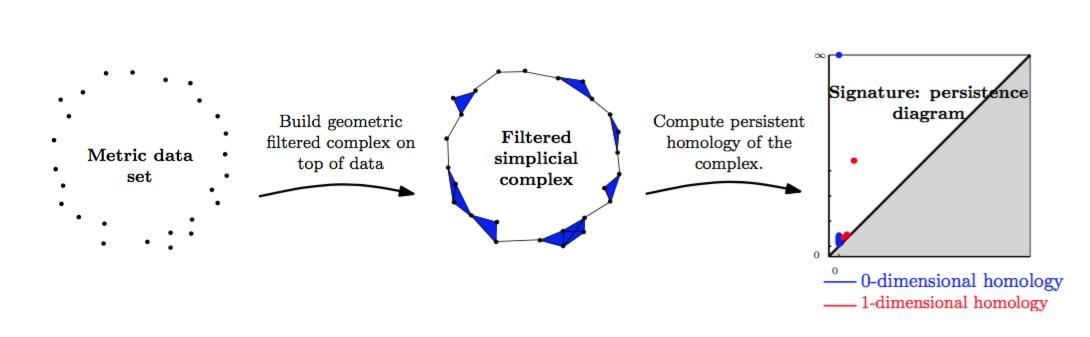
\includegraphics[width=130mm]{img/tda-workflow.jpeg}
	\caption{text}
\end{figure}

El TDA ofrece una perspectiva única que es invaluable en numerosos campos donde la forma y la conectividad de los datos son esenciales para entender procesos complejos. Esta herramienta no solo mejora nuestra capacidad para analizar conjuntos de datos complejos, sino que también facilita la detección de patrones y estructuras subyacentes significativas en diversas aplicaciones prácticas y teóricas.


\endinput
%--------------------------------------------------------------------
% FIN DEL CAPÍTULO. 
%--------------------------------------------------------------------
